\chapter{Data and simulated samples}\label{chap:datamc}

\section{Data}\label{sec:datamc:data}
The analysis presented in this thesis is performed on \emph{\protonproton} collision data collected by ATLAS and delivered by the LHC Run-2, between 2015 and 2018, corresponding to a total integrated luminosity of \SI{139}{\femto\barn^{-1}}. The breakdown of the luminosity collected in each year by ATLAS available for physics analysis is outlined in \cref{tab:data:lumi}. The luminosity uncertainty is determined from calibration of the luminosity scale using the Van Der Meer scans described in \cref{sec:method:lumi}. 
\begin{table}[h]
    \centering
    \begin{tabular}{l|c}
        Year & luminosity [\SI{}{\femto\barn^{-1}}] \\
        \hline
        2015 & 3.2 \\
        2016 & 33.0 \\
        2017 & 44.3 \\
        2018 & 59.9 \\
        \hline 
        \hline
        Total & 139 $\pm$ 1.7\% \\
	\end{tabular}
    \caption[Summary of the luminosities of datasets taken between 2015 and 2018]{Summary of the luminosities of datasets taken between 2015 and 2018~\cite{ATLAS:lumiPlots}.}
    \label{tab:data:lumi}
  \end{table}

~\cref{fig:yields2015,fig:yields2016,fig:yields2017,fig:yields2018} show the data yeilds (events per [\SI{}{\pico\barn^{-1}}) after applying the analysis selection for different data taking periods during the runs between 2015 to 2018. 

\begin{figure}[ht]
\centering
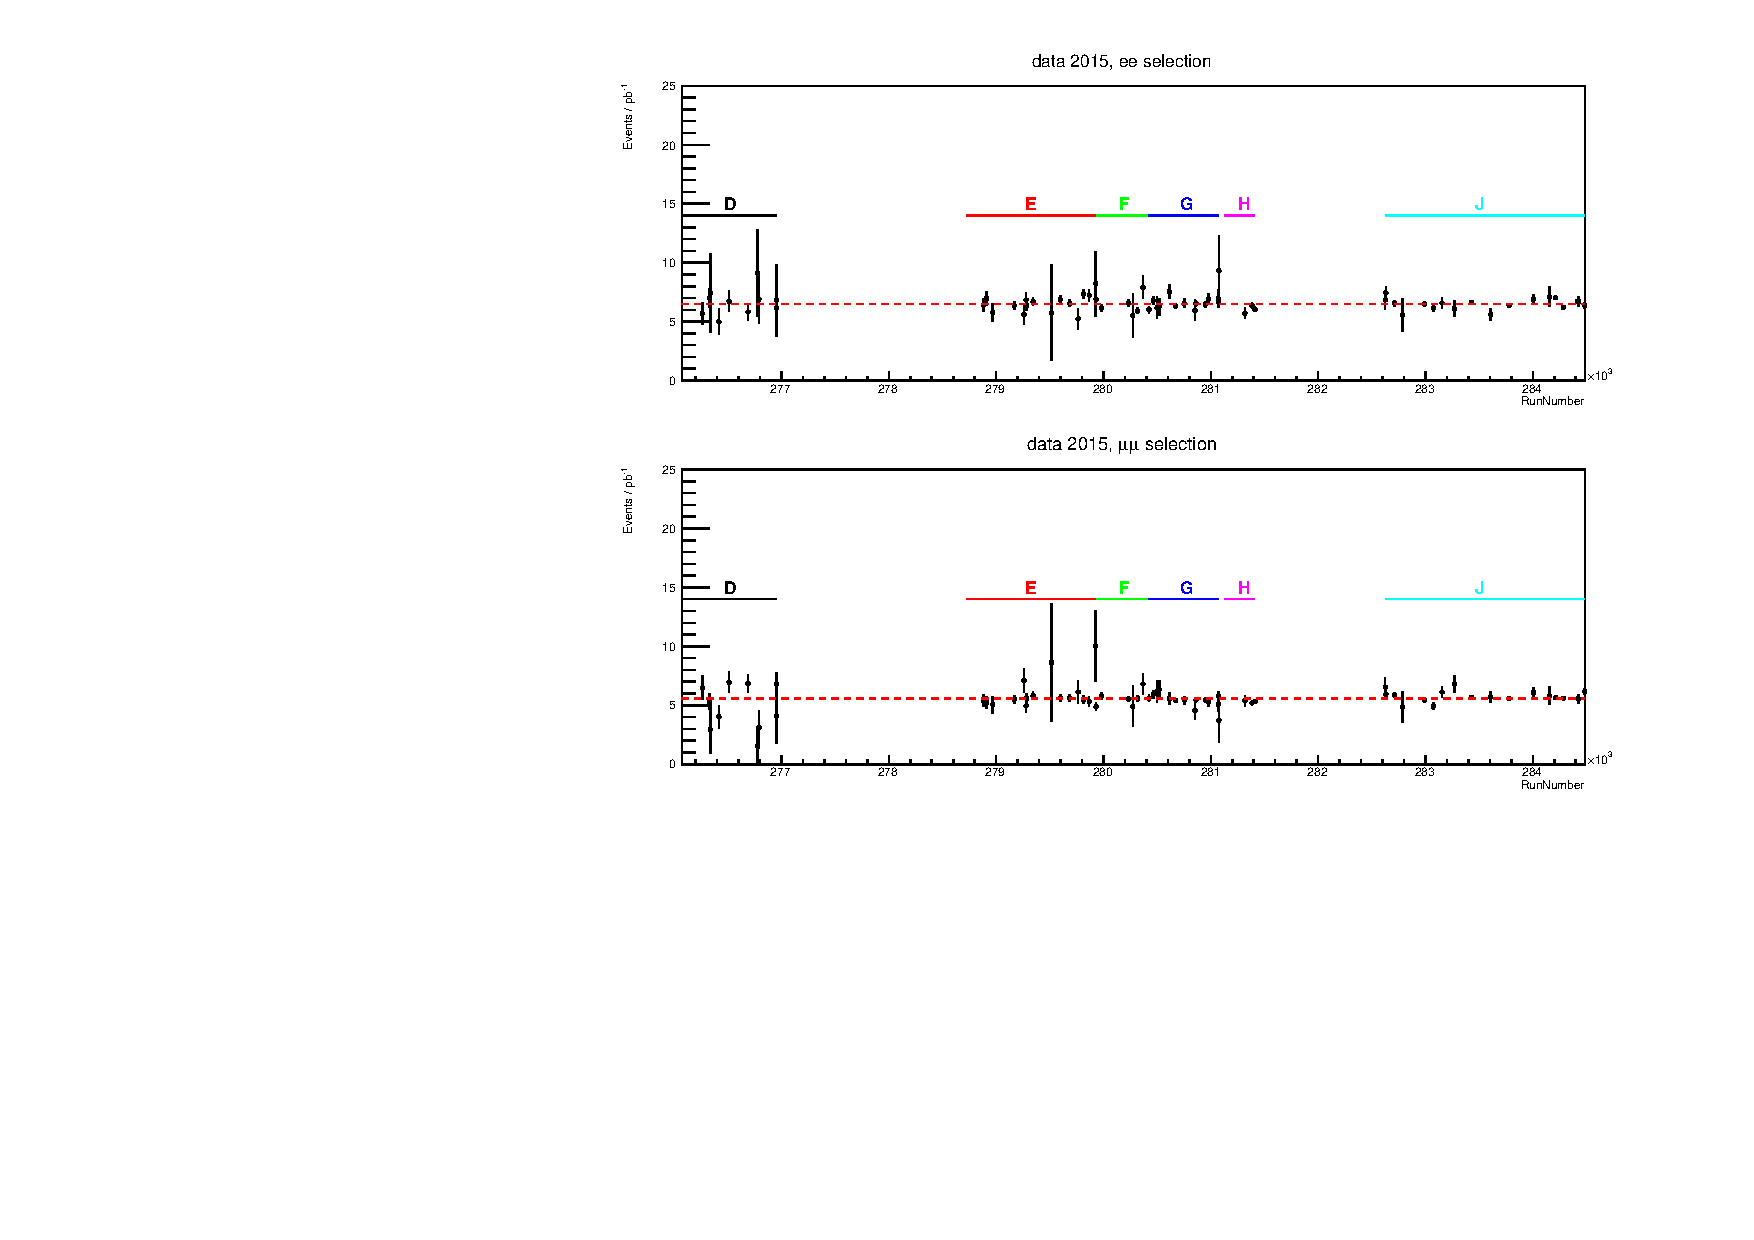
\includegraphics[width=\textwidth]{figures/analysis/datamc/Yields/compare_data_yields2015.pdf}
\caption[Data yields for the 2015 run period for the $ee$ (above) and $\mu\mu$ (below) selections.]{Data yields for the 2015 run period for the $ee$ (above) and $\mu\mu$ (below) selections. Each letter on the legend correspond to the different data taking periods within a year~\cite{Aad:2019fac}.}
\label{fig:yields2015}
\end{figure}

\begin{figure}[ht]
\centering
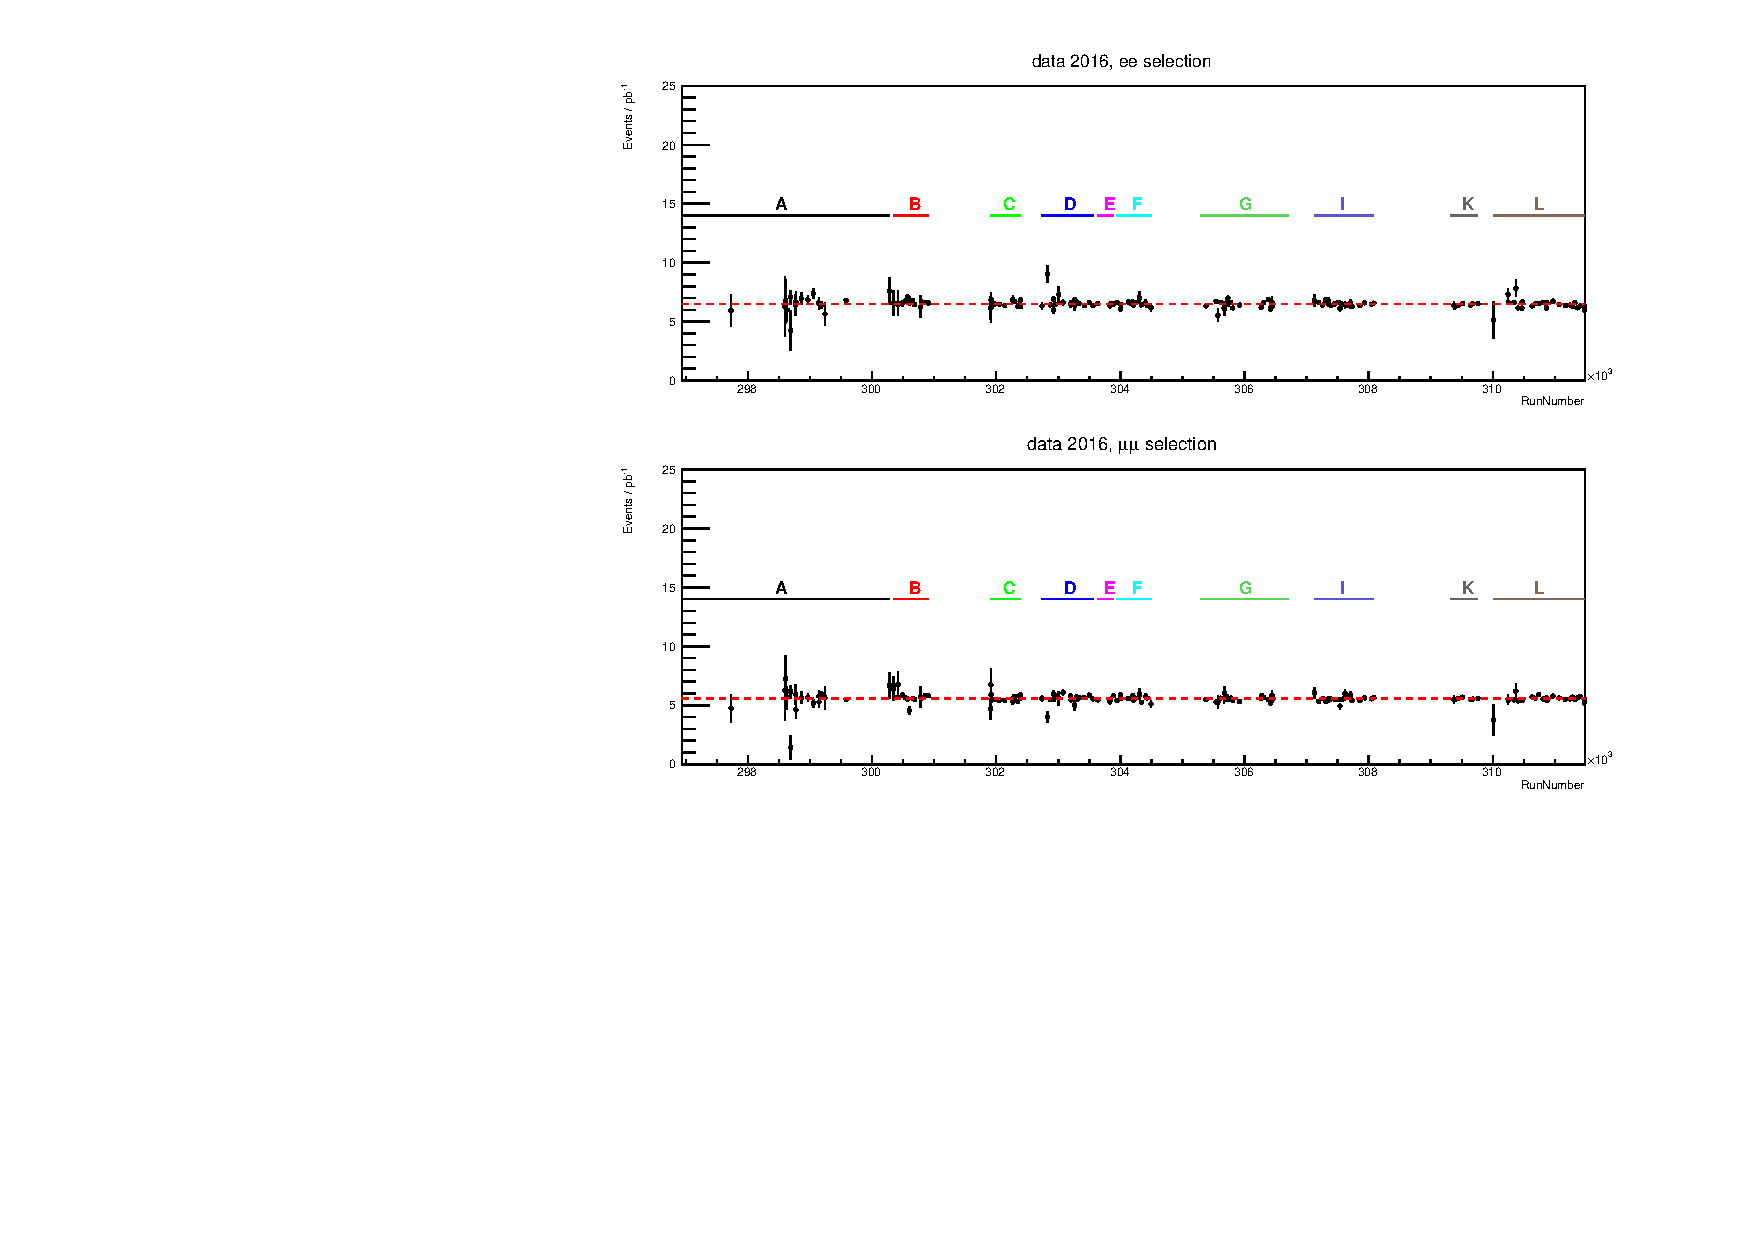
\includegraphics[width=\textwidth]{figures/analysis/datamc/Yields/compare_data_yields2016.pdf}
\caption[Data yields for the 2016 run period for the $ee$ (above) and $\mu\mu$ (below) selections.]{Data yields for the 2016 run period for the $ee$ (above) and $\mu\mu$ (below) selections. Each letter on the legend correspond to the different data taking periods within a year~\cite{Aad:2019fac}.}
\label{fig:yields2016}
\end{figure}

\begin{figure}[ht]
\centering
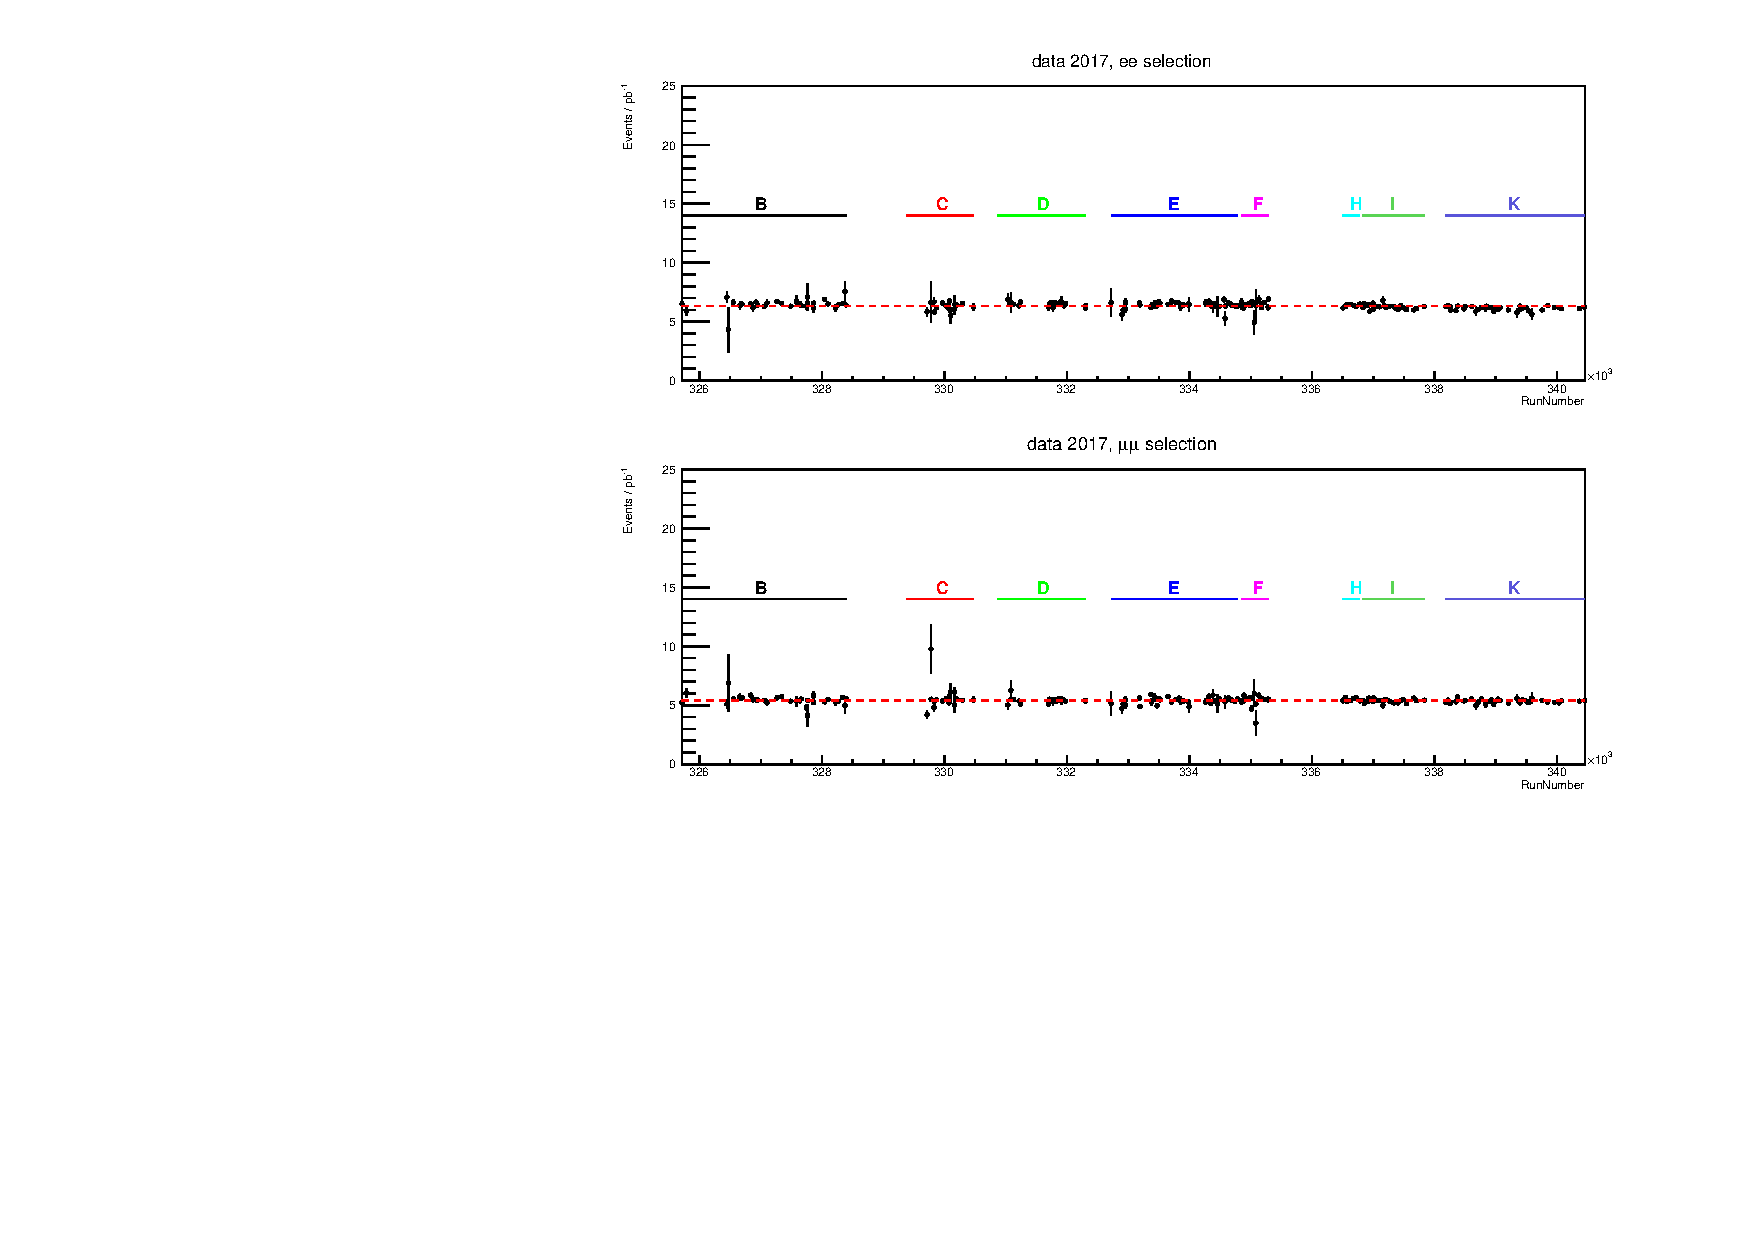
\includegraphics[width=\textwidth]{figures/analysis/datamc/Yields/compare_data_yields2017.pdf}
\caption[Data yields for the 2017 run period for the $ee$ (above) and $\mu\mu$ (below) selections.]{Data yields for the 2017 run period for the $ee$ (above) and $\mu\mu$ (below) selections. Each letter on the legend correspond to the different data taking periods within a year~\cite{Aad:2019fac}.}
\label{fig:yields2017}
\end{figure}

\begin{figure}[ht]
\centering
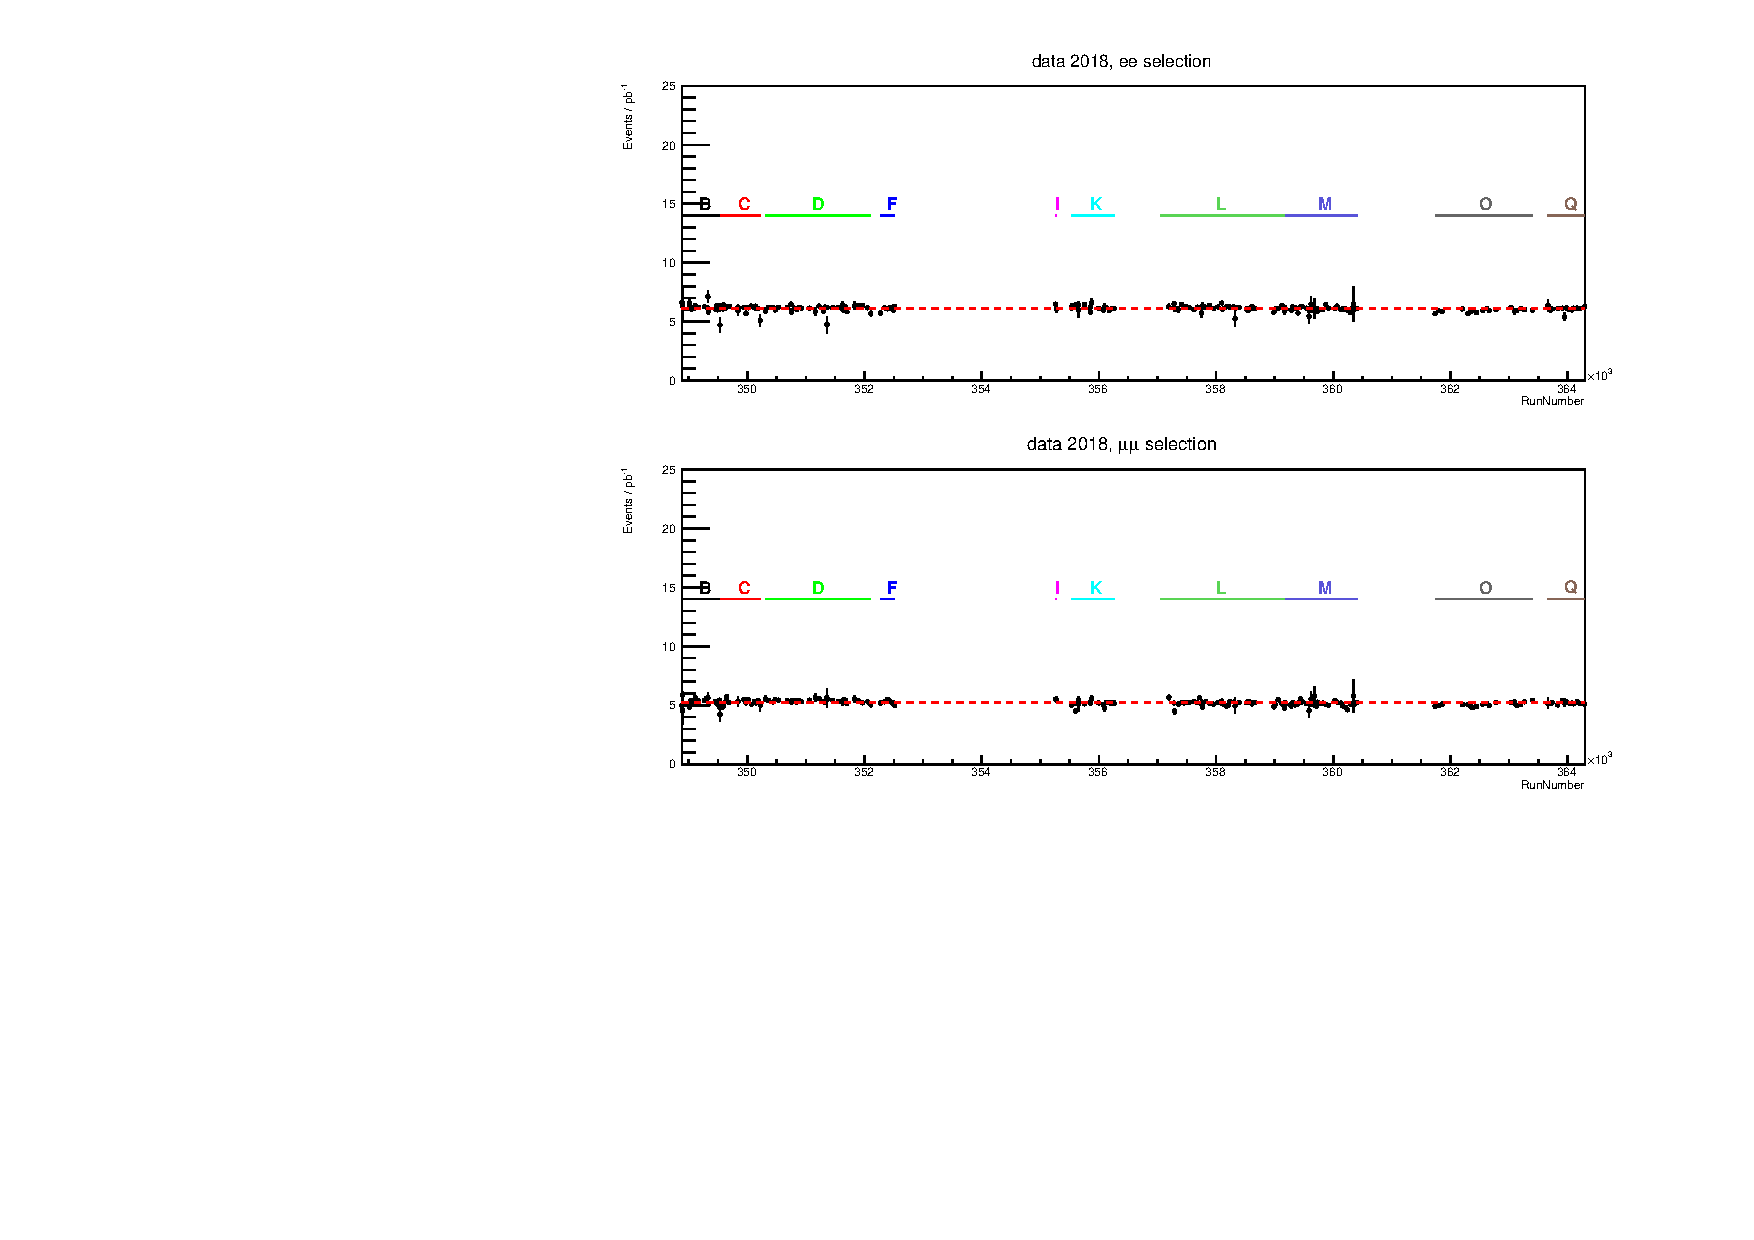
\includegraphics[width=\textwidth]{figures/analysis/datamc/Yields/compare_data_yields2018.pdf}
\caption[Data yields for the 2018 run period for the $ee$ (above) and $\mu\mu$ (below) selections.]{Data yields for the 2018 run period for the $ee$ (above) and $\mu\mu$ (below) selections Each letter on the legend correspond to the different data taking periods within a year~\cite{Aad:2019fac}.}
\label{fig:yields2018}
\end{figure}

\clearpage

\section{Monte Carlo samples}\label{sec:datamc:mc}
While the analysis is carried out in a data driven way, simulated samples for the background and signal are used to determine the appropriate functional form to fit the data, study background compositions, estimate uncertainties and evaluate signal. This section outlines the MC samples used for the background and signal samples.

While generators are available to produce events using higher order matrix elements are now available, it is often required to enhance the description of the process beyond the order of the generator used. Higher order QCD and EW corrections can modify the shape of the invariant mass distributions. Mass-dependent \emph{K}-factors can be derived taking the ratio of the higher order differential cross-section calculation over the available sample, e.g. next-to-next-to-leading order(NNLO) over the next-to-leading order (NLO). The \emph{K}-factors can then be applied to the invariant mass distribution on an event by event basis to produce higher order samples. 

Simulated samples include the effects of pileup interactions, performed with \PYTHIAV{v8.186} using the ATLAS A3 set of tuned parameters~\cite{ATL-PHYS-PUB-2016-017} and the NNPDF23LO PDF set, and weighted accordingly to the number of pileup interactions observed in data. The simulated samples then pass through the full detector simulation as described in \cref{sec:simulation}. 

\subsection{Background samples}\label{sec:datamc:mc:bkg}
The main backgrounds in decreasing order of importance are Drell-Yan (DY), top-quark ($t\bar{t}$), single-top-quark and diboson production. For the electron channel is it prohibitive to produce MC with enough events to accurately represent the expected QCD multijet distribution, due to the very small probabilities of jets faking electrons which pass the analysis selection. Therefore, the QCD and W+Jets processes in the dielectron channel are estimated with a data driven method~\cite{EXOT-2016-05}. For the muon channel the multijet background was studied and found to be negligible~\cite{EXOT-2016-05}, therefore, the contribution is neglected. 

The SM Drell-Yan process is modelled using the NLO \POWHEGBOX~\cite{Alioli:2010xd,Frixione:2007vw} event generator using the CT10 PDF~\cite{ct10} together with \PYTHIAV{v8.186}~\cite{pythia8} is used for event showering. The DY samples are generated in slices of dilepton invariant mass, where 19 mass-binned samples were created with dilepton invariant mass ranging from \SI{120}{\giga\electronvolt} and $>$ \SI{5000}{\giga\electronvolt}, to increase the statistics of the samples in the high-mass regions. Corrections are applied to the DY samples to correct them from NLO to NNLO using using a mass dependent \emph{K}-factor is calculated with {\textsc{VRAP}} v0.9~\cite{vrap} and the CT14 NNLO PDF set~\cite{CT14} for QCD effects. {\textsc{MCSANC}}~\cite{MCSANC} is used for quantum electrodynamic corrections.  The diboson processes ($WW$, $WZ$ and $ZZ$) are generated at NLO using \SHERPA 2.1.1~\cite{Gleisberg:2008ta} with the CT10 PDF. Similar to the DY samples, the diboson samples were generated in invariant mass slices to increase the statistics of the sample. The $t\bar{t}$ background is generated at NLO using \POWHEGBOX with the NNPDF3.0NLO~\cite{Ball:2014uwa} PDF. Single top (s/t-channel) uses \POWHEGBOX with NNPDF3.0NLO PDF. A top quark mass of \SI{175.2}{\giga\electronvolt} is set for the generation of these samples. The top quark samples are normalised to the cross section at NNLO in QCD including resummation of the NNLO leading order soft gluon terms as provided by \textsc{Top++}2.0~\cite{Czakon:2011xx}.

The MC event generators for the hard-scattering process, showering and PDFs are listed in \cref{tab:MC}. A detailed description of the event simulation procedure is given in \cref{sec:simulation}. "Afterburner" generators such as \textsc{Photos}~\cite{Golonka:2005pn} for the final-state photon radiation (FSR) modelling, \textsc{MadSpin}~\cite{Artoisenet:2012st} to preserve top-quark spin correlations, and \textsc{EvtGen}~\cite{Lange:2001uf}, used for the modelling of $c$- and $b$-hadron decays, are also included in the simulation.

\begin{table}[htbp]
\centering
\tablesize{
\begin{tabular}{llp{5cm}}
\toprule
Background Process & ME Generator and ME PDFs & PS and non-perturbative effect with PDFs \\\hline
NLO Drell--Yan & \POWHEGBOX~\cite{Alioli:2010xd,Frixione:2007vw}, CT10~\cite{ct10}, \textsc{Photos} & \PYTHIAV{v8.186}~\cite{pythia8}, CTEQ6L1~\cite{ATL-PHYS-PUB-2014-021,Stump:2003yu}, \newline \textsc{EvtGen1.2.0} \\
$t\bar{t}$  & \POWHEGBOX, NNPDF3.0NLO~\cite{Ball:2014uwa} & \PYTHIAV{v8.230}, NNPDF23LO~\cite{Ball:2012cx}, \newline \textsc{EvtGen1.6.0} \\
Single top $s$-channel, $Wt$& \POWHEGBOX, NNPDF3.0NLO & \PYTHIAV{v8.230}, NNPDF23LO, \newline \textsc{EvtGen1.6.0} \\
Single top $t$-channel & \POWHEGBOX, NNPDF3.04fNLO, \textsc{MadSpin} & \PYTHIAV{v8.230}, NNPDF23LO,\newline  \textsc{EvtGen1.6.0}  \\
Diboson ($WW$, $WZ$ and $ZZ$) & \SHERPA 2.1.1~\cite{Gleisberg:2008ta}, CT10 &\SHERPA 2.1.1, CT10  \\\hline
Signal Process & & \\\hline
LO Drell--Yan & \PYTHIAV{v8.186}, NNPDF23LO  &  \PYTHIAV{v8.186}, NNPDF23LO, \newline \textsc{EvtGen1.2.0} \\
LO CI & \PYTHIAV{v8.186}, NNPDF23LO  &  \PYTHIAV{v8.186}, NNPDF23LO, \newline \textsc{EvtGen1.2.0} \\
\bottomrule
\end{tabular}
}
\caption[The event generators used for PDFs and generating matrix element (ME) and parton shower (PS) simulation of the signal and background processes.]{The event generators used for PDFs and generating matrix element (ME) and parton shower (PS) simulation of the signal and background processes. The top-quark mass is set to \SI{175.2}{\giga\electronvolt}.}
\label{tab:MC}
\end{table}

\subsection{Signal samples}\label{sec:datamc:mc:sig}
The \PYTHIAV{v8.230} generator is used to produce CI signal samples at leading-order (LO) using the NNPDF23LO PDF. Five benchmark values of $\Lambda$ from 10-\SI{30}{\tera\electronvolt} in steps of \SI{5}{\tera\electronvolt} were generated for each of the CI models. The CI shapes contain both the SM DY background and the interference between the DY and CI. 

It is possible to reweight the SM background to BSM signals when both the signal and background have the same initial and final states, due to  SM background particles being required as inputs for BSM signal+background differential cross sections. Therefore, an event dependent reweighting factor can be derived by taking the ratio of the SM and BSM (e.g CI) differential cross sections on an event by event basis. The reweighting scale factor is given by~\cite{EXOT-2016-05}:
\begin{equation}
    S = \frac{\frac{d\sigma}{d\hat{t}}(q\bar{q} \rightarrow \gamma, CI \rightarrow f\bar{f})}{\frac{d\sigma}{d\hat{t}}(q\bar{q} \rightarrow \gamma, Z \rightarrow f\bar{f})},
\end{equation}
where the numerator refers the BSM differential cross section and the denominator refers to the SM process only. It is possible to reweight any SM kinematic quantities to the correspond BSM one using this method as the differential cross sections are functions of event kinematics. This technique circumvents the requirement to generate MC samples for each potential signal hypothesis that needs to be tested, but, rather allowing for samples to be generated for any model by reweighting from a single background sample. 

Leading-order (LO) DY samples generated using \PYTHIAV{v8.186} with NNPDF23LO PDF is used in the reweighting procedure. The weights are applied to the LO DY events to transform into CI signal shapes, in steps of \SI{2}{\tera\electronvolt} between $\Lambda = \SI{12}{\tera\electronvolt}$ and $\Lambda = \SI{100}{\tera\electronvolt}$. In addition, dilepton mass dependent higher-order QCD and electroweak production corrections for signals are computed with the same methodology as for the DY background. While higher order QCD corrections are expected to be the same for signals and background, it is not clear the electroweak corrections can be treated the same. The addition of the electroweak corrections may be less conservative, however, it is deemed to be closer to the theoretically correct treatment than being over conservative and not including the corrections. 

The dedicated CI samples are used to validate the reweighting procedure, \cref{fig:datamc:sigValidate} shows an example of a CI mass slice between between 3000 - \SI{4000}{\giga\electronvolt} where the reweighted CI interaction sample and the dedicated sample is compared. \cref{fig:datamc:sigoverlays} shows the invariant mass distributions for for constructive and destructive interference models reweighted using the procedure described above. 

\begin{figure}[h]
    \centering
    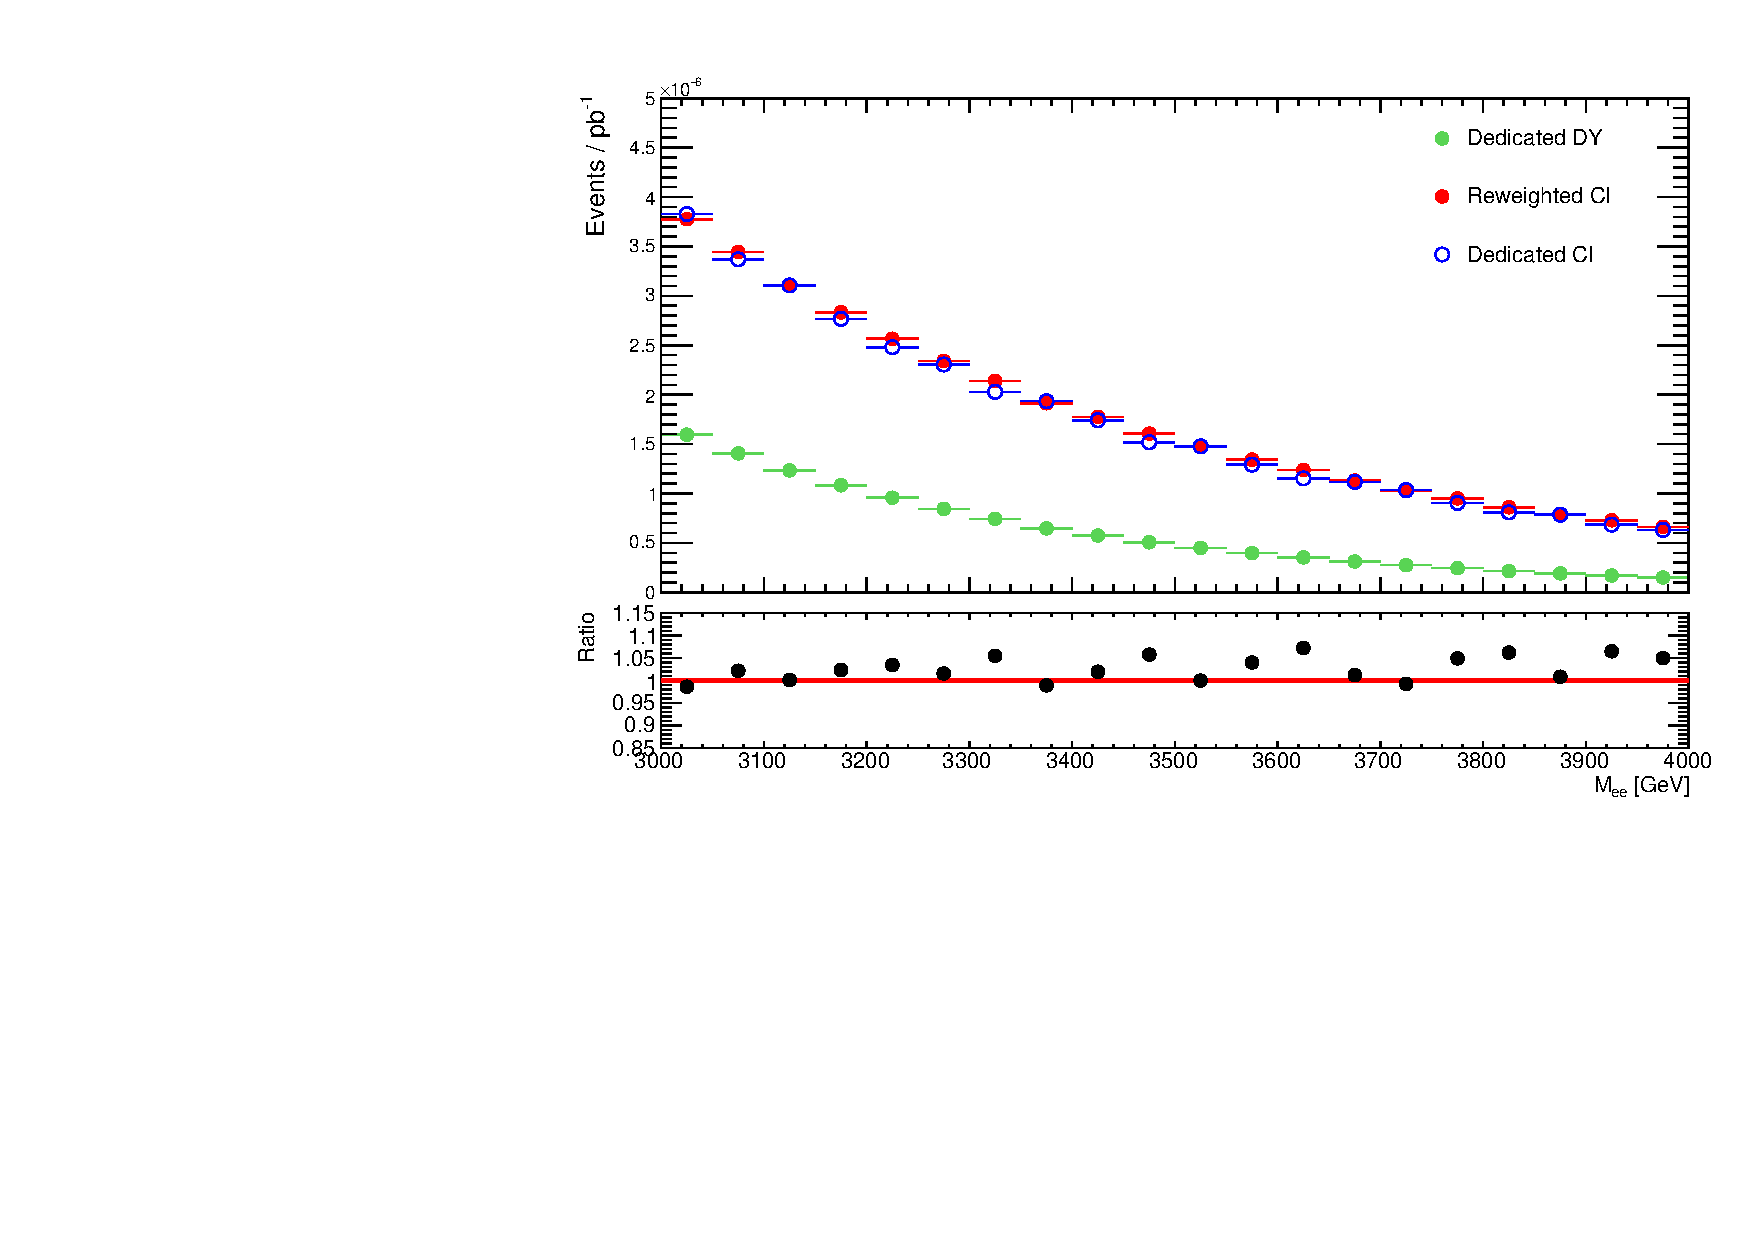
\includegraphics[width=\mediumfigwidth]{figures/analysis/datamc/sigmodel/CICompare.pdf}
    \caption[Validation of signal reweighting]{Comparison of dedicated and reweighted CI sample in the invariant mass range from 3000 - \SI{4000}{\giga\electronvolt} is shown in the top pad. The DY sample used to reweight is also shown. The bottom pad shows the ratio between the reweighted and dedicated CI signal.}
    \label{fig:datamc:sigValidate}
\end{figure}

\begin{figure}[]
    \centering
    \begin{subfigure}[b]{0.49\textwidth}
        \centering
        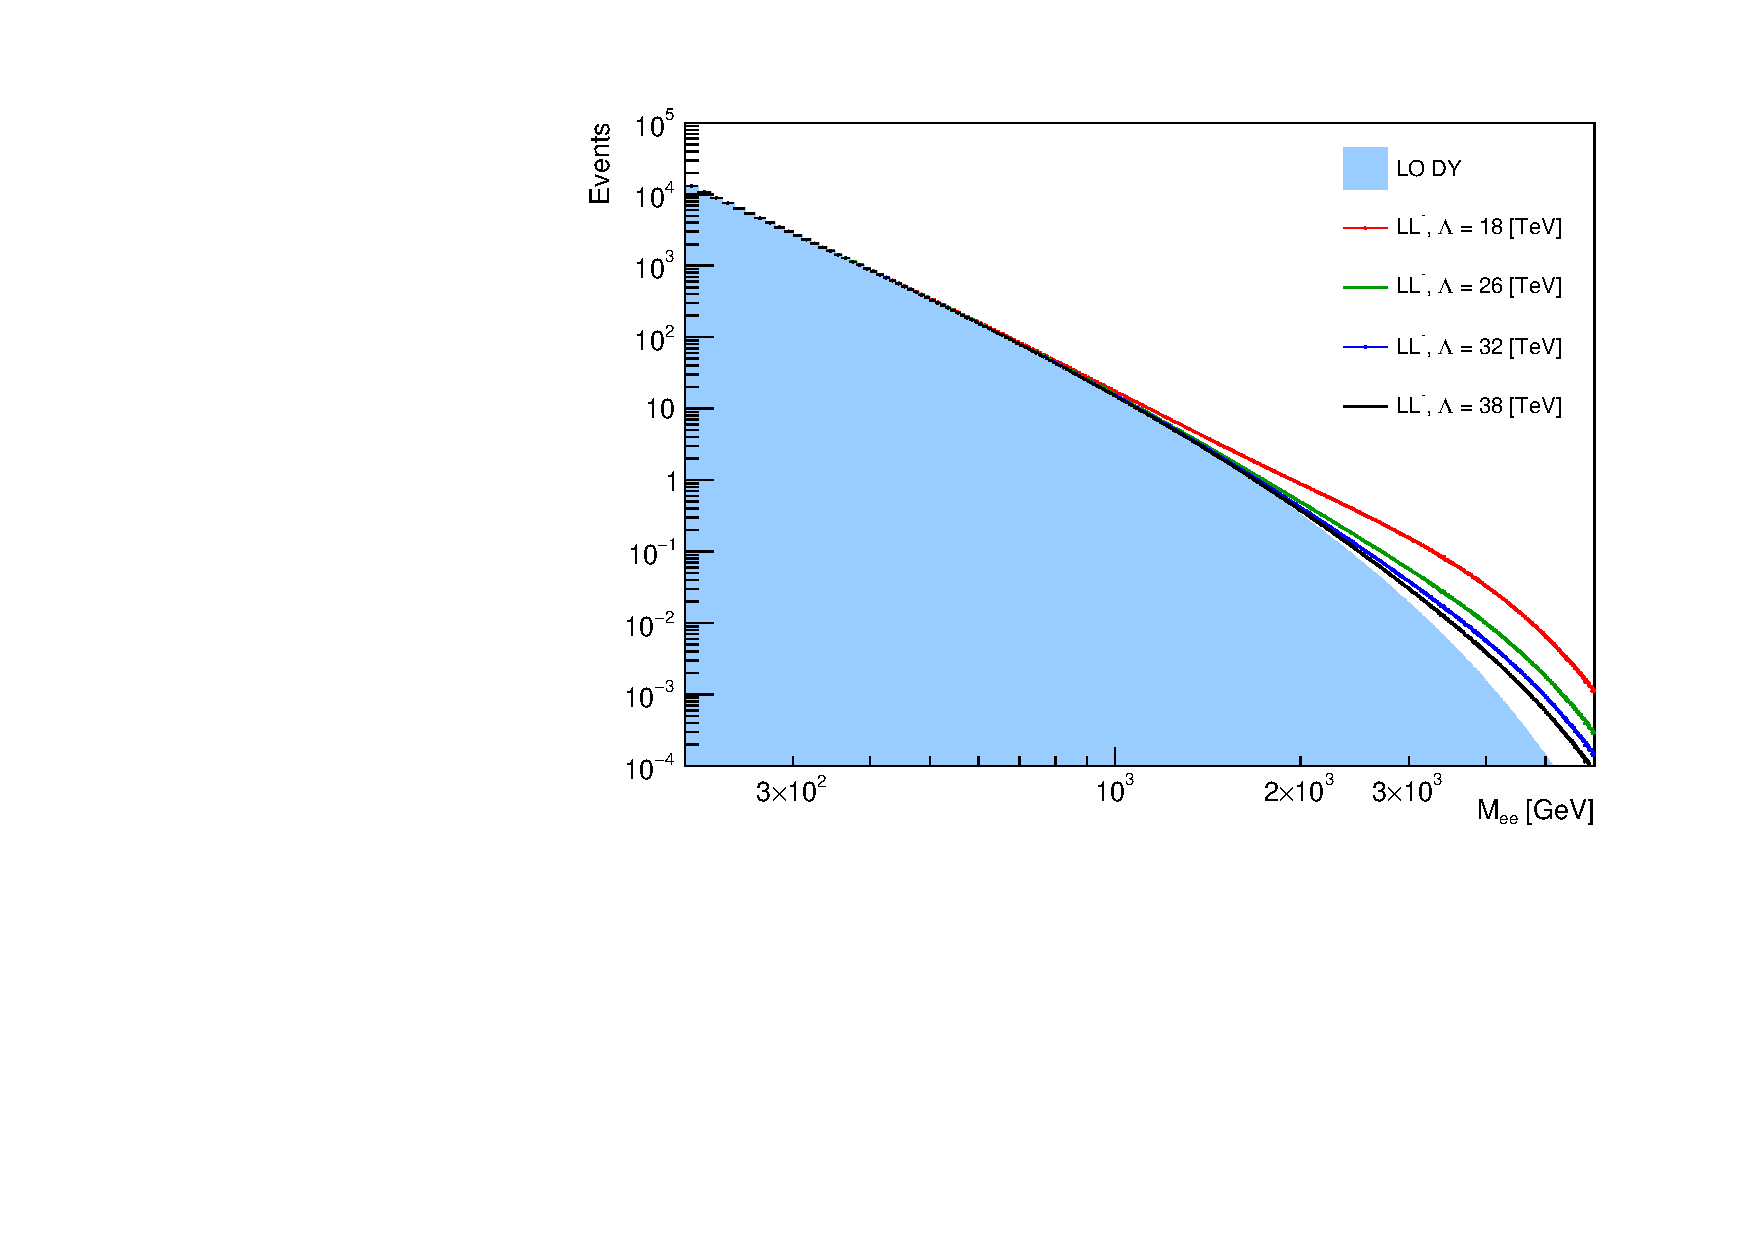
\includegraphics[width=\textwidth]{figures/analysis/datamc/sigmodel/constSigsOverlay.pdf}
        \caption{}
        \label{fig:datamc:sigconstoverlays}
    \end{subfigure}
    \begin{subfigure}[b]{0.49\textwidth}
        \centering
        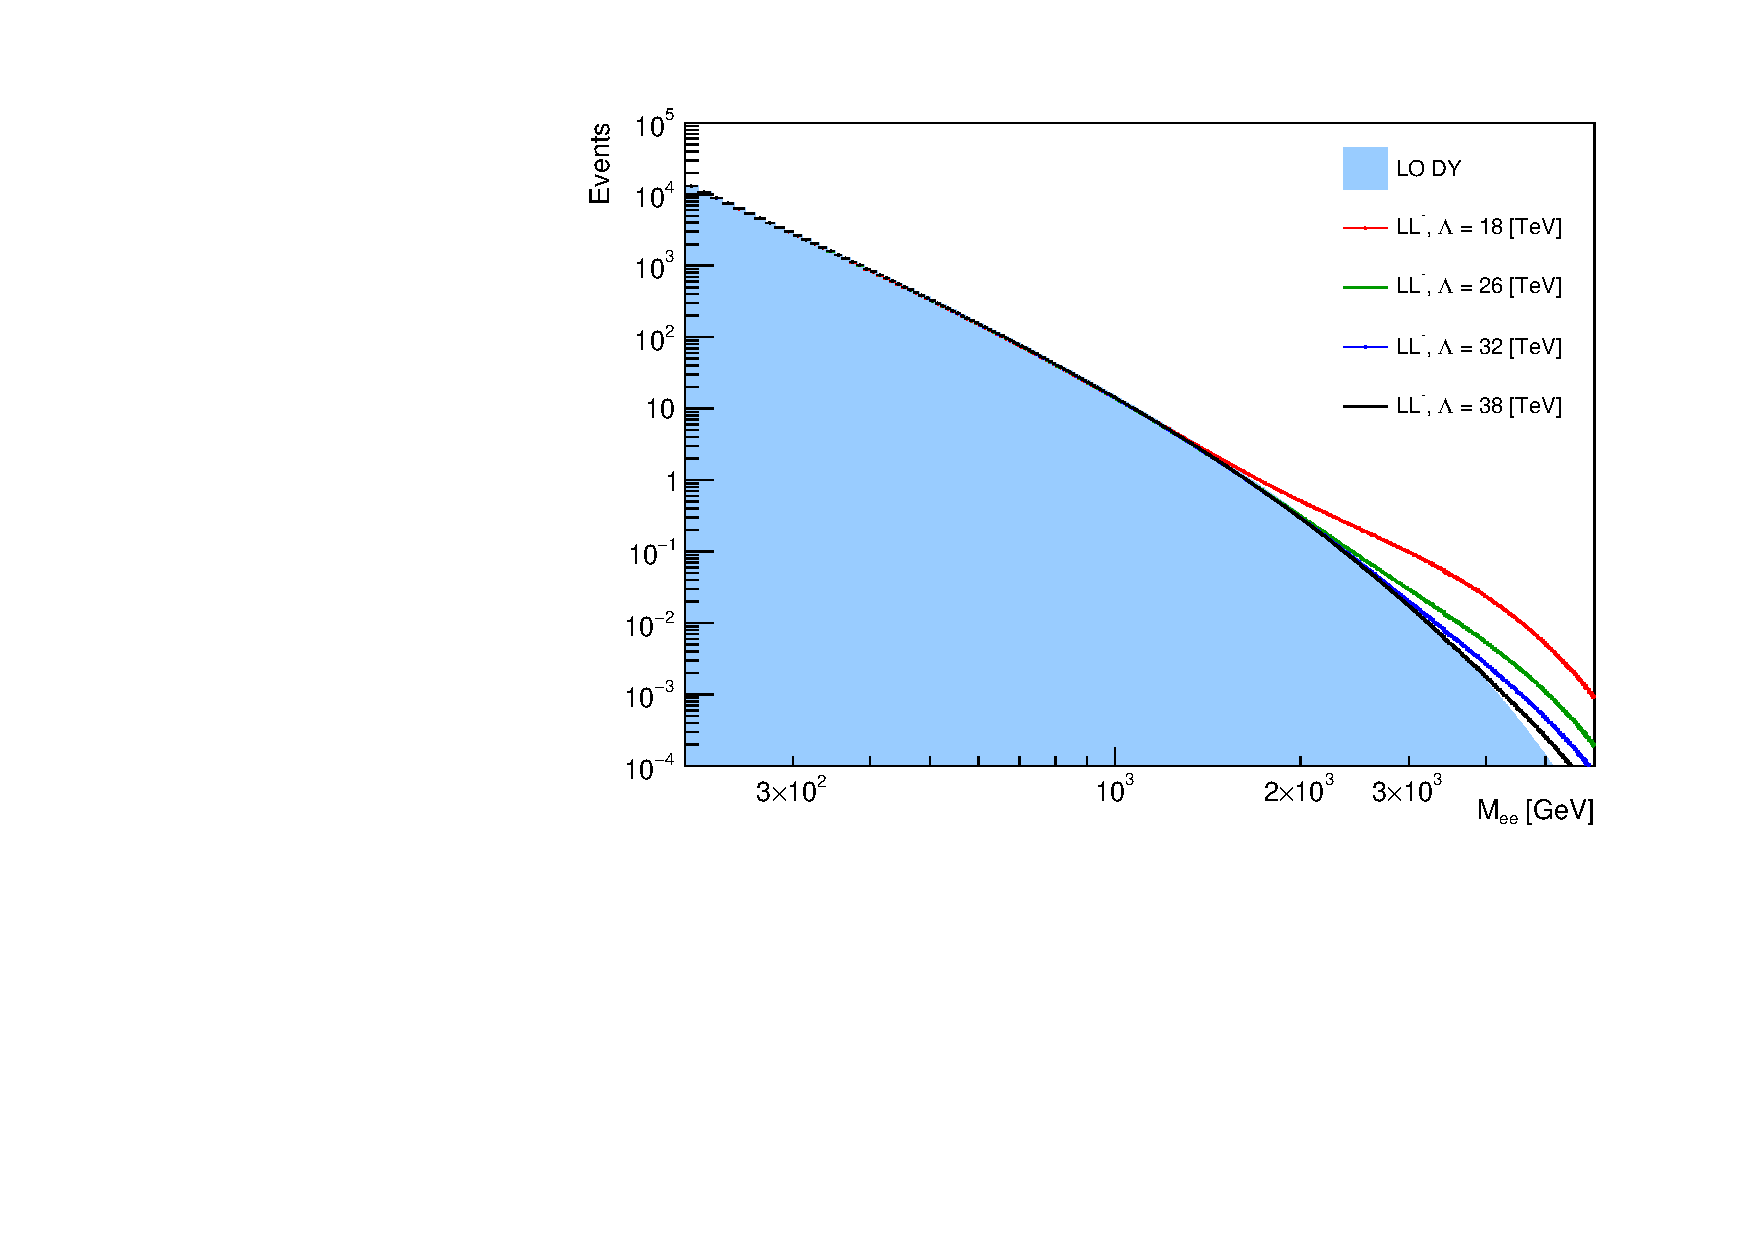
\includegraphics[width=\textwidth]{figures/analysis/datamc/sigmodel/destSigsOverlay.pdf}
        \caption{}
        \label{fig:datamc:sigdestoverlays}
    \end{subfigure}
    \caption[Invariant mass distribution for reweighted CI LL signal models]{Invariant mass distributions for LL constructive (a) and destructive (b) CI interaction models with the DY sample used to reweight it. The interference of the CI interaction is shown by the + (constructive) and - (destructive) sign on the legend.}
    \label{fig:datamc:sigoverlays}
\end{figure}

\section{Estimation of fake background}\label{sec:datamc:fakes}
Processes involving jets or electron and a jet can pass the signal event selection of the signature of the jets are reconstructed as electrons. The electron plus jet final state are mainly due to W+Jets processes. Typically light-flavour jets, containing charged and neutral pions are misidentified as electrons during reconstruction. Due to the high energies of collisions at the LHC the decays of neutral pions, $\pi^0 \rightarrow \gamma\gamma$, are highly boosted and can lead to narrow electromagnetic energy depositions. These processes can give rise to signatures that are difficult to distinguish from those of the desired electrons. The desired leptons are referred to as "real electrons", whereas the mimicking leptons are referred to as \emph{fake electrons}. The fake background is difficult to estimate using simulation, therefore data-driven techniques are often used. 

\subsection{Matrix method}
The analysis uses the likelihood matrix method~\cite{Varnes:2016nrb} to estimate the fake background contribution using two levels of electron identification criteria: a \emph{tight} (T) selection which corresponds to the nominal analysis selection, and a \emph{loose} (L) identification criteria which relaxes the nominal identification. The set of objects passing the \emph{tight} selection, $N_{tight}$, is a subset of those passing the \emph{loose} selection, $N_{loose}$. Pairs of electron candidates are considered denoted by $N_{xy}$ with $x,y \in t,l$, giving the number of electron pairs passing a specific selection. The fist index representing the leading electron ($p_{T,lead} > p_{T,sublead}$) and the second one the subleading electron. An additional set of quantities $N_{xy}$ with $x,y \in R,F$ can be defined to denote whether an electron is real (R) or fake (F). The relationship between the two sets of quantities can be given by~\cite{EXOT-2016-05}:

\begin{equation}\label{eq:matrix_method_1}
\left(\begin{array}{c}N_{TT}\\ N_{TL}\\ N_{LT}\\ N_{LL}\end{array}\right) = M \left(\begin{array}{c}N_{RR}\\ N_{RF}\\ N_{FR}\\ N_{FF}\end{array}\right) , M =
    \begin{pmatrix}
    r_1r_2 & r_1f_2 &  f_1r_2 & f_1f_2\\
    r_1\tilde{r2} & r_1\tilde{f2} & f_1\tilde{r2} & f_1\tilde{f2}\\
    \tilde{r1}r_2 & \tilde{r1}f_2 & \tilde{f1}r_2 & \tilde{f1}f_2\\
    \tilde{r1}\tilde{r2} & \tilde{r1}\tilde{f2} & \tilde{f1}\tilde{r2} & \tilde{f1}\tilde{f2}  
    \end{pmatrix}
\end{equation}

where $\tilde{x} = 1 - x$. The vectors on the right (left) hand side contain exclusive measurable (not measurable) quantities, e.g L would denote a electron that passes the \emph{loose} selection and not the tight selection. The coefficients r and f correspond to the real and fake rates respectively. The real efficiency is the probability of real electrons to be reconstructed as \emph{tight} electrons and is calculated using MC, whereas the fake efficiency is the probability of a fake electron to be selected as \emph{loose} to be reconstructed as a \emph{tight} electron and is calculated on data. The index 1 and 2 correspond to the efficiencies of the leading and subleading electrons. 

To estimate the number of misidentified events within the electron selection, the number of events passing the signal selection ($N_{TT}$), which contain at least one fake object must be measured. These fake events arise from events where at least one electron is misidentified (RF and FR) or both electrons are misidentified (RR). The total number of fake electrons can be obtained from the sum of these contributions:

\begin{equation}
    \begin{aligned}\label{eq:mm:nfakes}
    & N^{\text{e+jet}}_{TT}=r_1f_2N_{RF}+f_1r_2N_{FR} ,\\ 
    & N^{\text{multijet}}_{TT}=f_1f_2N_{FF} ,\\ 
    & N^{\text{fake}}_{TT}=r_1f_2N_{RF}+f_1r_2N_{FR}+f_1f_2N_{FF} ,
    \end{aligned}
\end{equation}

A likelihood is formed to include poisson constraints on $N_{xy}$ with $x,y \in T,L$:
\begin{equation}
    \mathcal{L} = \prod_{x,y \in T,L} P(N_{xy},N_{xy}^{pred}), 
\end{equation}
where \emph{P} represents the Poisson constraint on the observed number of events in each lepton category and is consistent with the predicted number of fake and real leptons. The predicted values can be expressed in terms of a linear combination of $N_{xy}$ with $x,y \in R,F$ terms by using \cref{eq:matrix_method_1}:
\begin{equation}
    \begin{aligned}
    N_{TL}^{pred} = (r_1r_2)N_{RR} + (r_1f_2)N_{RF} + (f_1r_2)N_{FR} + (f_1f_2)N_{RR},  \\
    N_{LT}^{pred} = (r_1\tilde{r_2})N_{RR} + (r_1\tilde{f_2})N_{RF} + (f_1\tilde{r_2})N_{FR} + (f_1\tilde{f_2})N_{RR}, \\
    N_{LL}^{pred} = (\tilde{r_1}\tilde{r_2})N_{RR} + (\tilde{r_1}\tilde{f_2})N_{RF} + (\tilde{f_1}\tilde{r_2})N_{FR} + (\tilde{f_1}\tilde{f_2})N_{RR}.
    \end{aligned}
\end{equation}

The Likelihood is then minimised the number of fakes can be extracted using \cref{eq:mm:nfakes}, which is them applied as an event by event weight used to produce an invariant mass distribution for the fake background contribution. The background template produced is then smoothed using a function fit~\cite{EXOT-2016-05}. 

\section{Data MC comparisons}\label{sec:datamc:compare}
\cref{fig:datamc:eecompare,fig:datamc:mmcompare} show the comparisons of the invariant mass distributions between the data and MC expectation with the addition of some benchmark CI interaction signals overlaid on top. The fake contribution is also included in the comparison. 
\cref{fig:datamc:pt1,fig:datamc:pt2} shows the \pt distribution for the leading and subleading leptons. The $\eta$ distributions for the leading and subleading leptons are shown in \cref{fig:datamc:eta1,fig:datamc:eta2}. In the electron channel the maximum can be seen at $\eta = 0$ and falls towards higher values of $\abs{\eta}$. The transition region coresponds to $1.37 < \abs{\eta} < 1.52$. The muon channel shows dips in the $\eta$ distributions in that correspond to poorly aligned chambers in the muon spectrometer. \cref{fig:datamc:phi1,fig:datamc:phi2} show the $\phi$ distributions for the leading and subleading leptons. A generally flat distribution can be seen in the electron channel. Small structures in the data are observed due to poor modelling of these in the background expectation, due to small inefficiencies in the identification in $\phi$ regions. The $\phi$ distribution for muons show small dips due to support structures on which the ATLAS detector is placed. 

\clearpage
\begin{figure}[]
    \centering
    \begin{subfigure}[b]{0.49\textwidth}
        \centering
        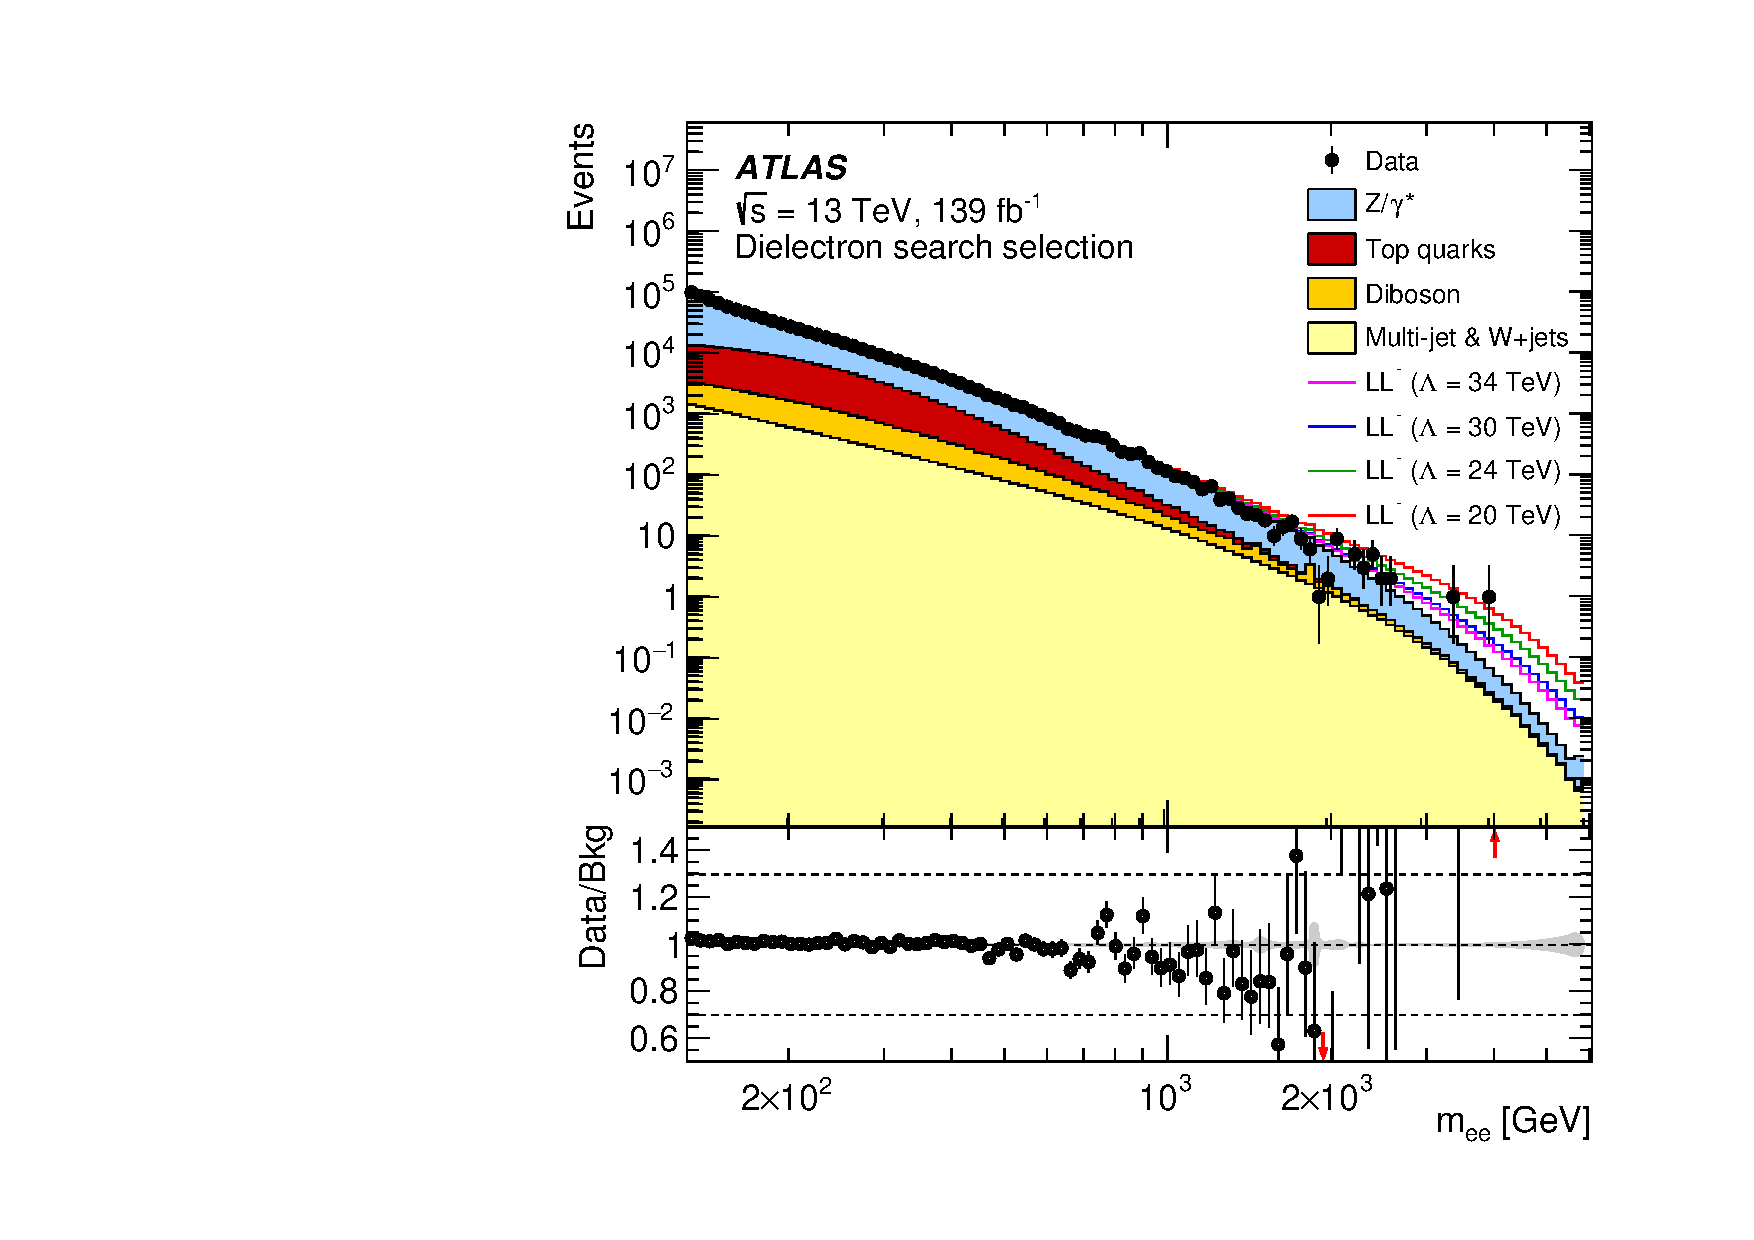
\includegraphics[width=\textwidth]{figures/analysis/datamc/dataMCcompare/const_ee_m_eebins_log100.pdf}
        \caption{}
        \label{fig:datamc:eeconst}
    \end{subfigure}
    \begin{subfigure}[b]{0.49\textwidth}
        \centering
        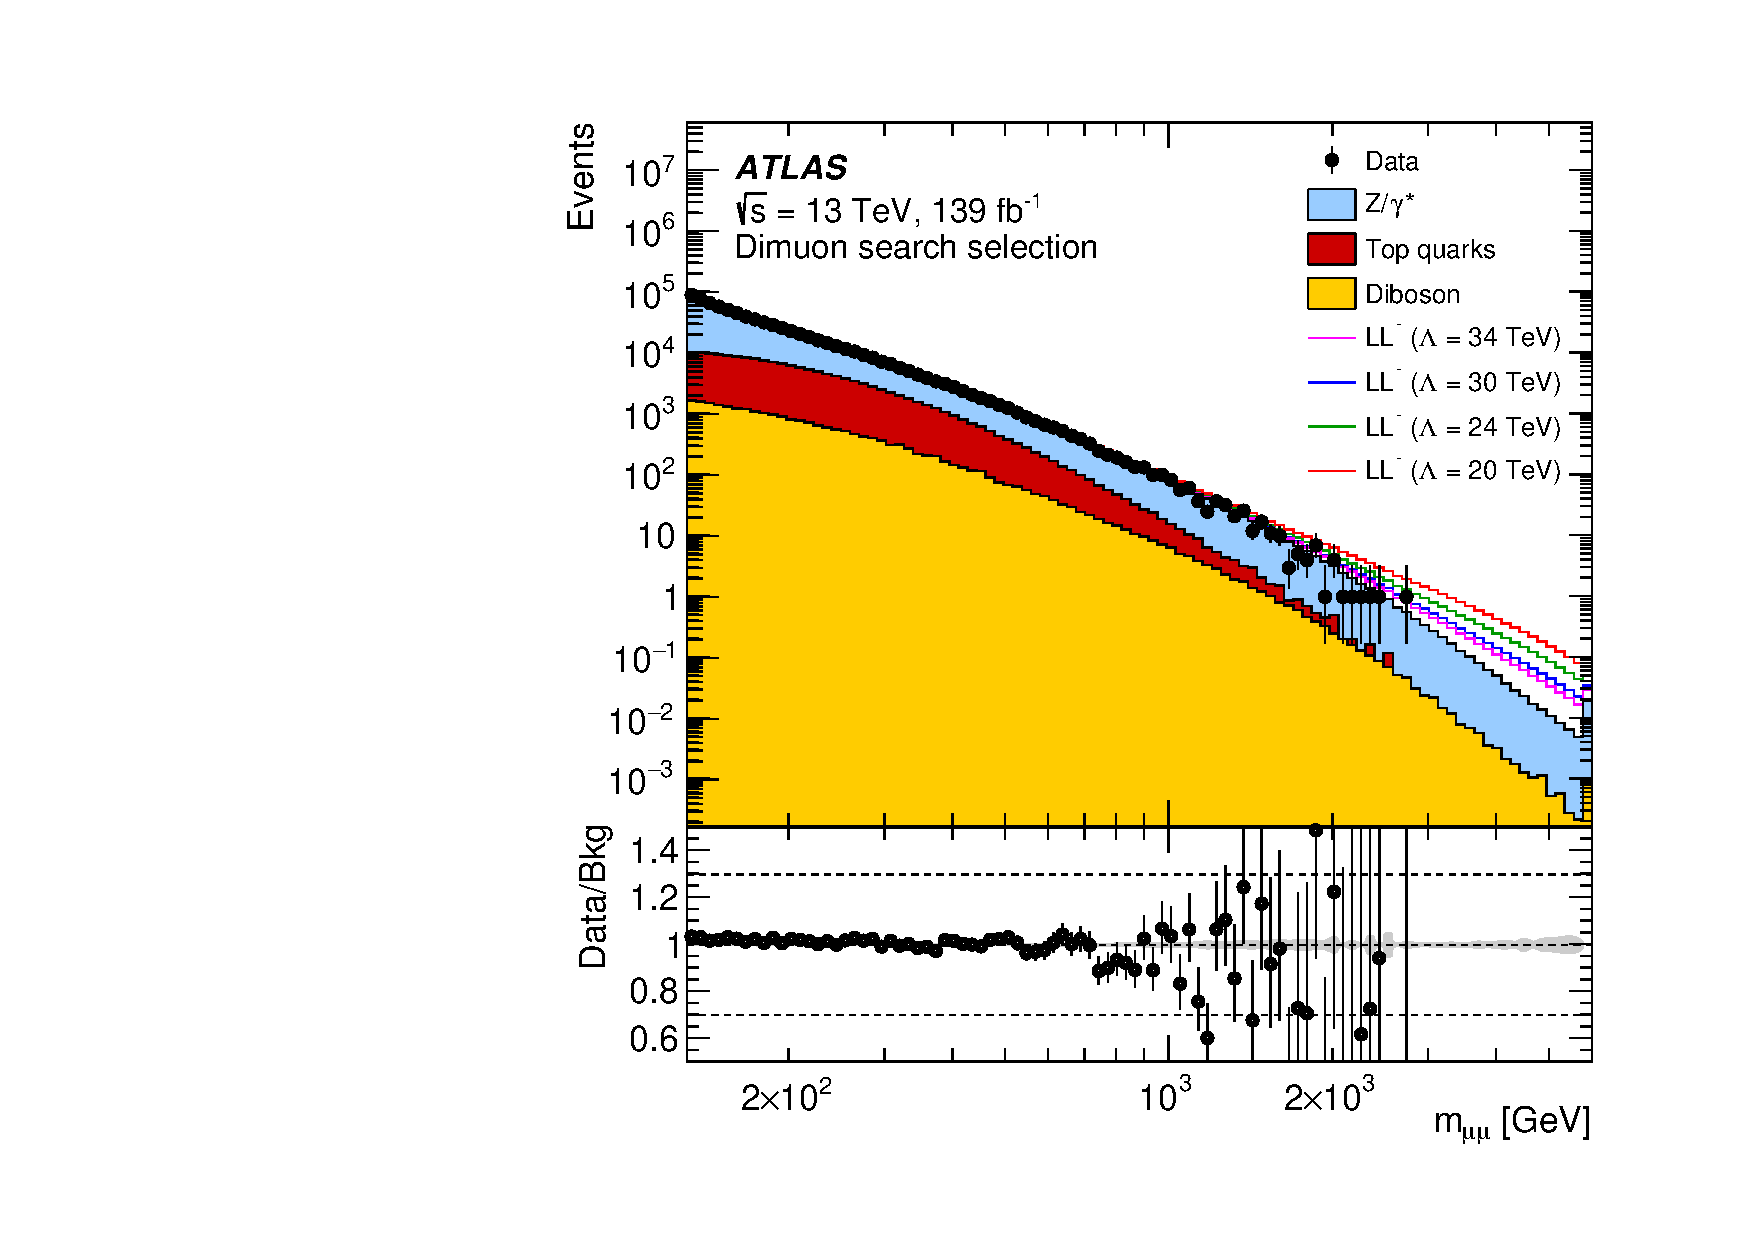
\includegraphics[width=\textwidth]{figures/analysis/datamc/dataMCcompare/const_uu_m_uubins_log100.pdf}
        \caption{}
        \label{fig:datamc:eedest}
    \end{subfigure}
    \caption[Invariant mass distributions for \ee channel]{Invariant mass distribution for the \ee selection for the full $2015-2018$ dataset and the respective MC campaign. The constructively interfering CI contributions are shown in (a),while destructive contributions are shown in (b).}
    \label{fig:datamc:eecompare}
\end{figure}

\begin{figure}[]
    \centering
    \begin{subfigure}[b]{0.49\textwidth}
        \centering
        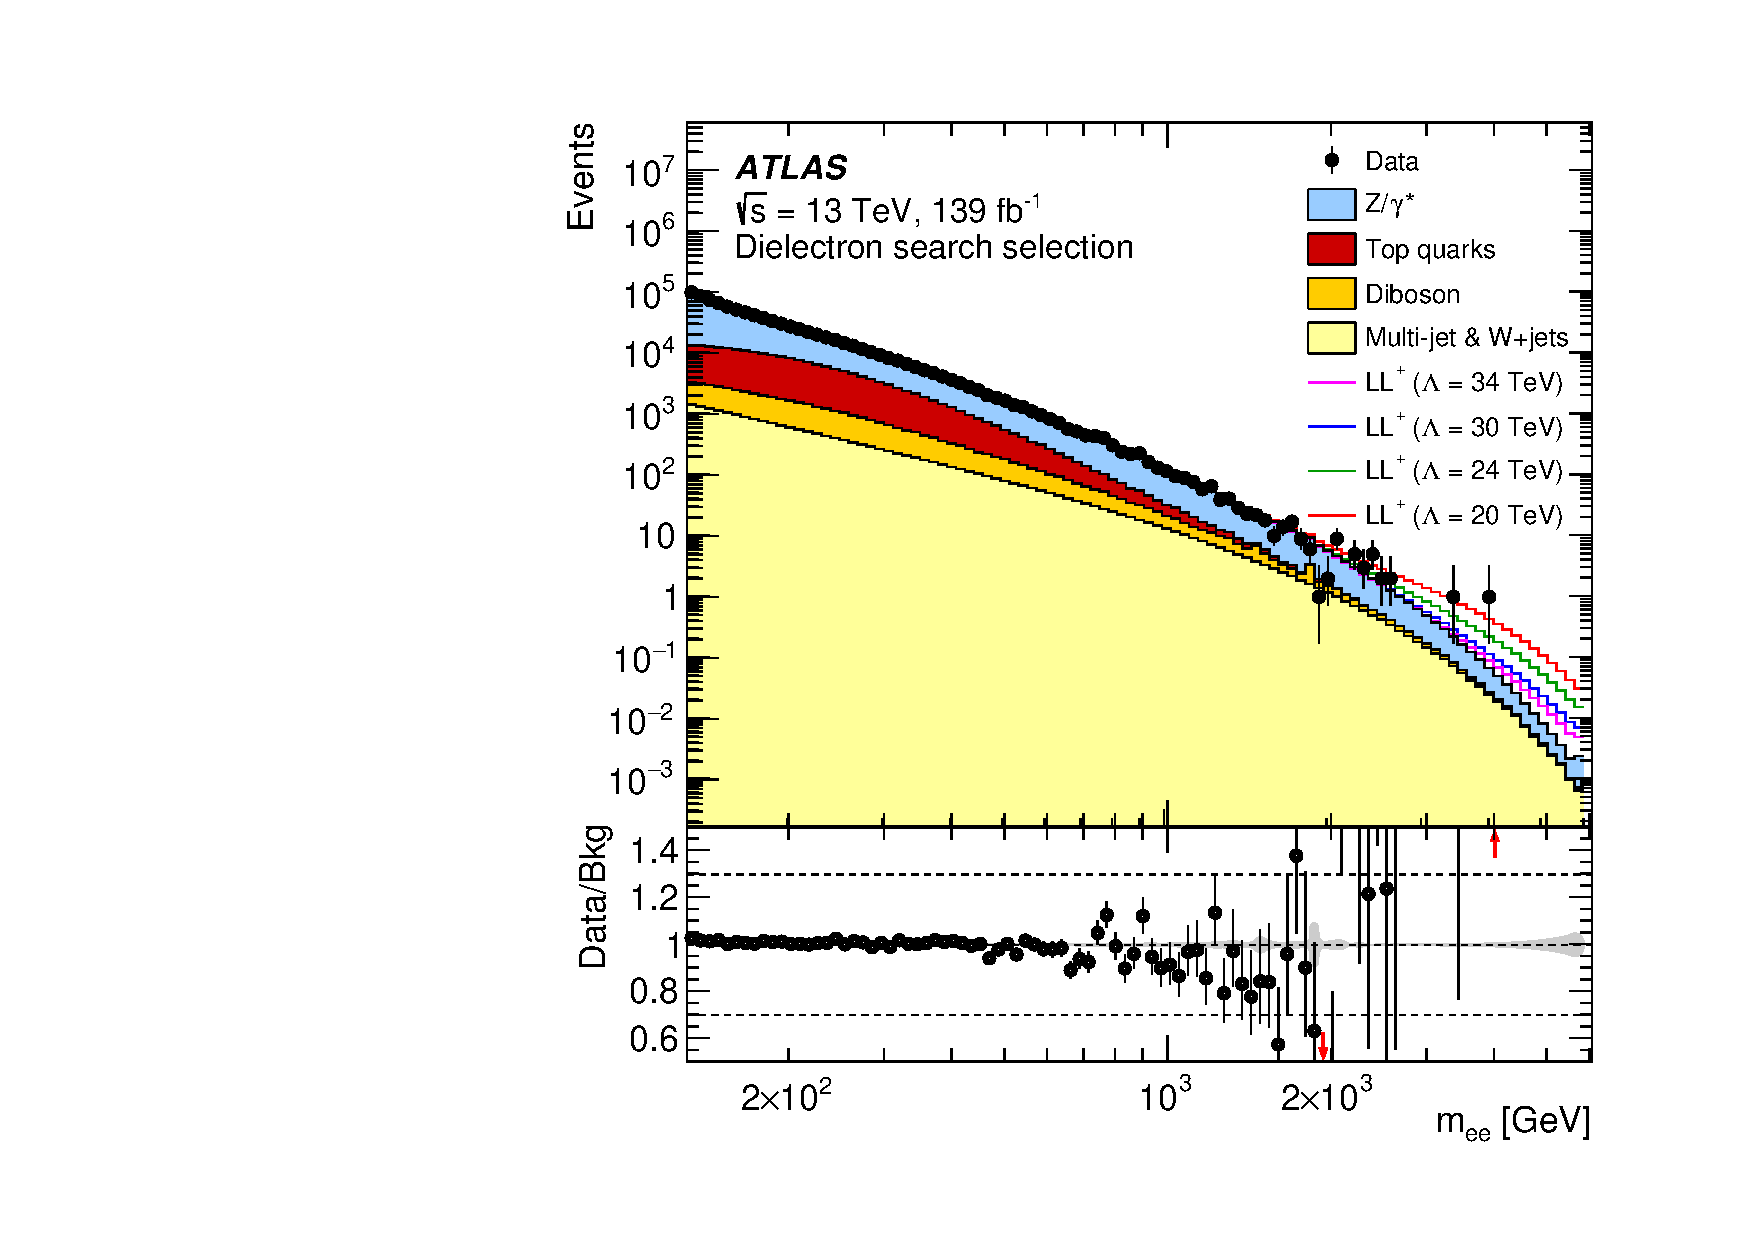
\includegraphics[width=\textwidth]{figures/analysis/datamc/dataMCcompare/dest_ee_m_eebins_log100.pdf}
        \caption{}
        \label{fig:datamc:mmconst}
    \end{subfigure}
    \begin{subfigure}[b]{0.49\textwidth}
        \centering
        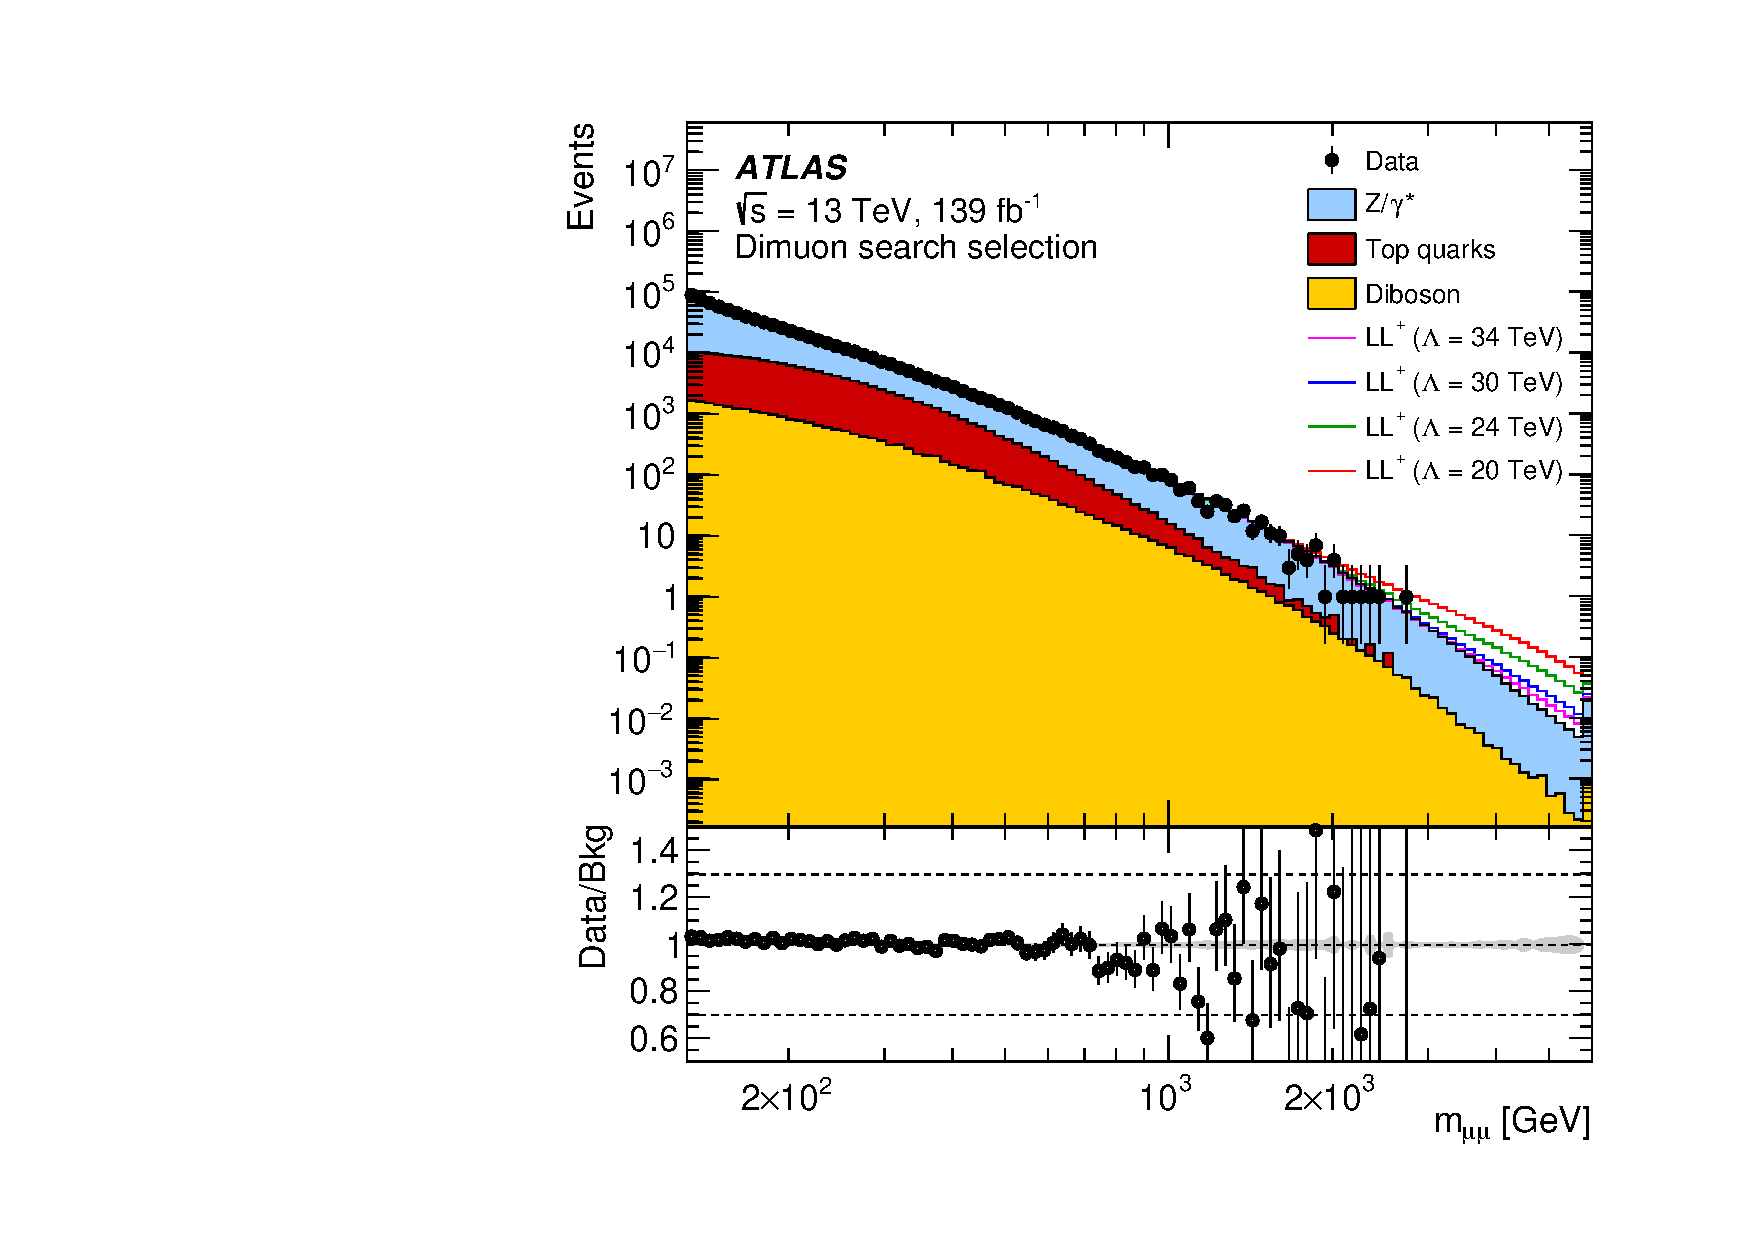
\includegraphics[width=\textwidth]{figures/analysis/datamc/dataMCcompare/dest_uu_m_uubins_log100.pdf}
        \caption{}
        \label{fig:datamc:mmdest}
    \end{subfigure}
    \caption[Invariant mass distributions for \mumu channel]{Invariant mass distribution for the \mumu selection for the full $2015-2018$ dataset and the respective MC campaign. The constructively interfering CI contributions are shown in (a), while destructive contributions are shown in (b).}
    \label{fig:datamc:mmcompare}
\end{figure}

\begin{figure}[]
    \centering
    \begin{subfigure}[b]{0.49\textwidth}
        \centering
        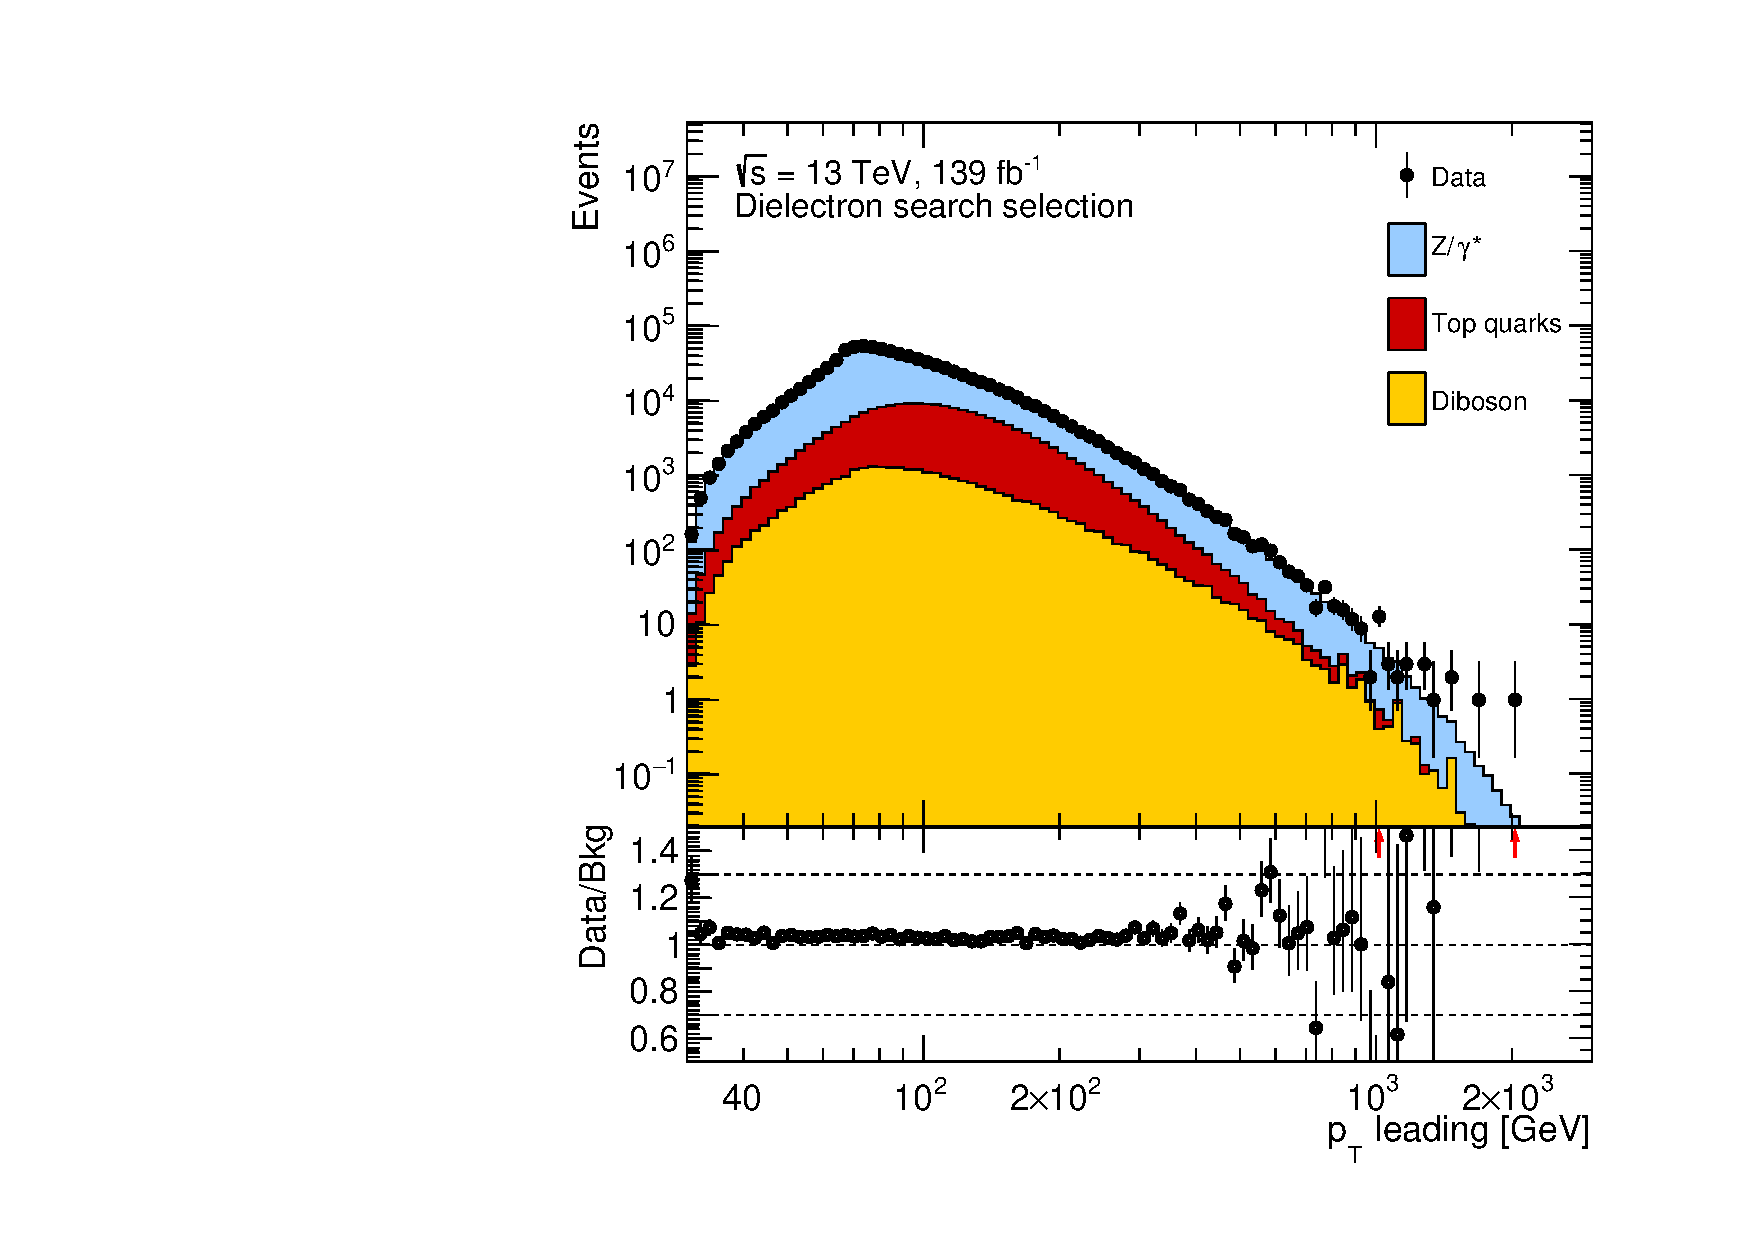
\includegraphics[width=\textwidth]{figures/analysis/datamc/dataMCcompare/ee_pt1_log100.pdf}
        \caption{}
        \label{fig:datamc:eept1}
    \end{subfigure}
    \begin{subfigure}[b]{0.49\textwidth}
        \centering
        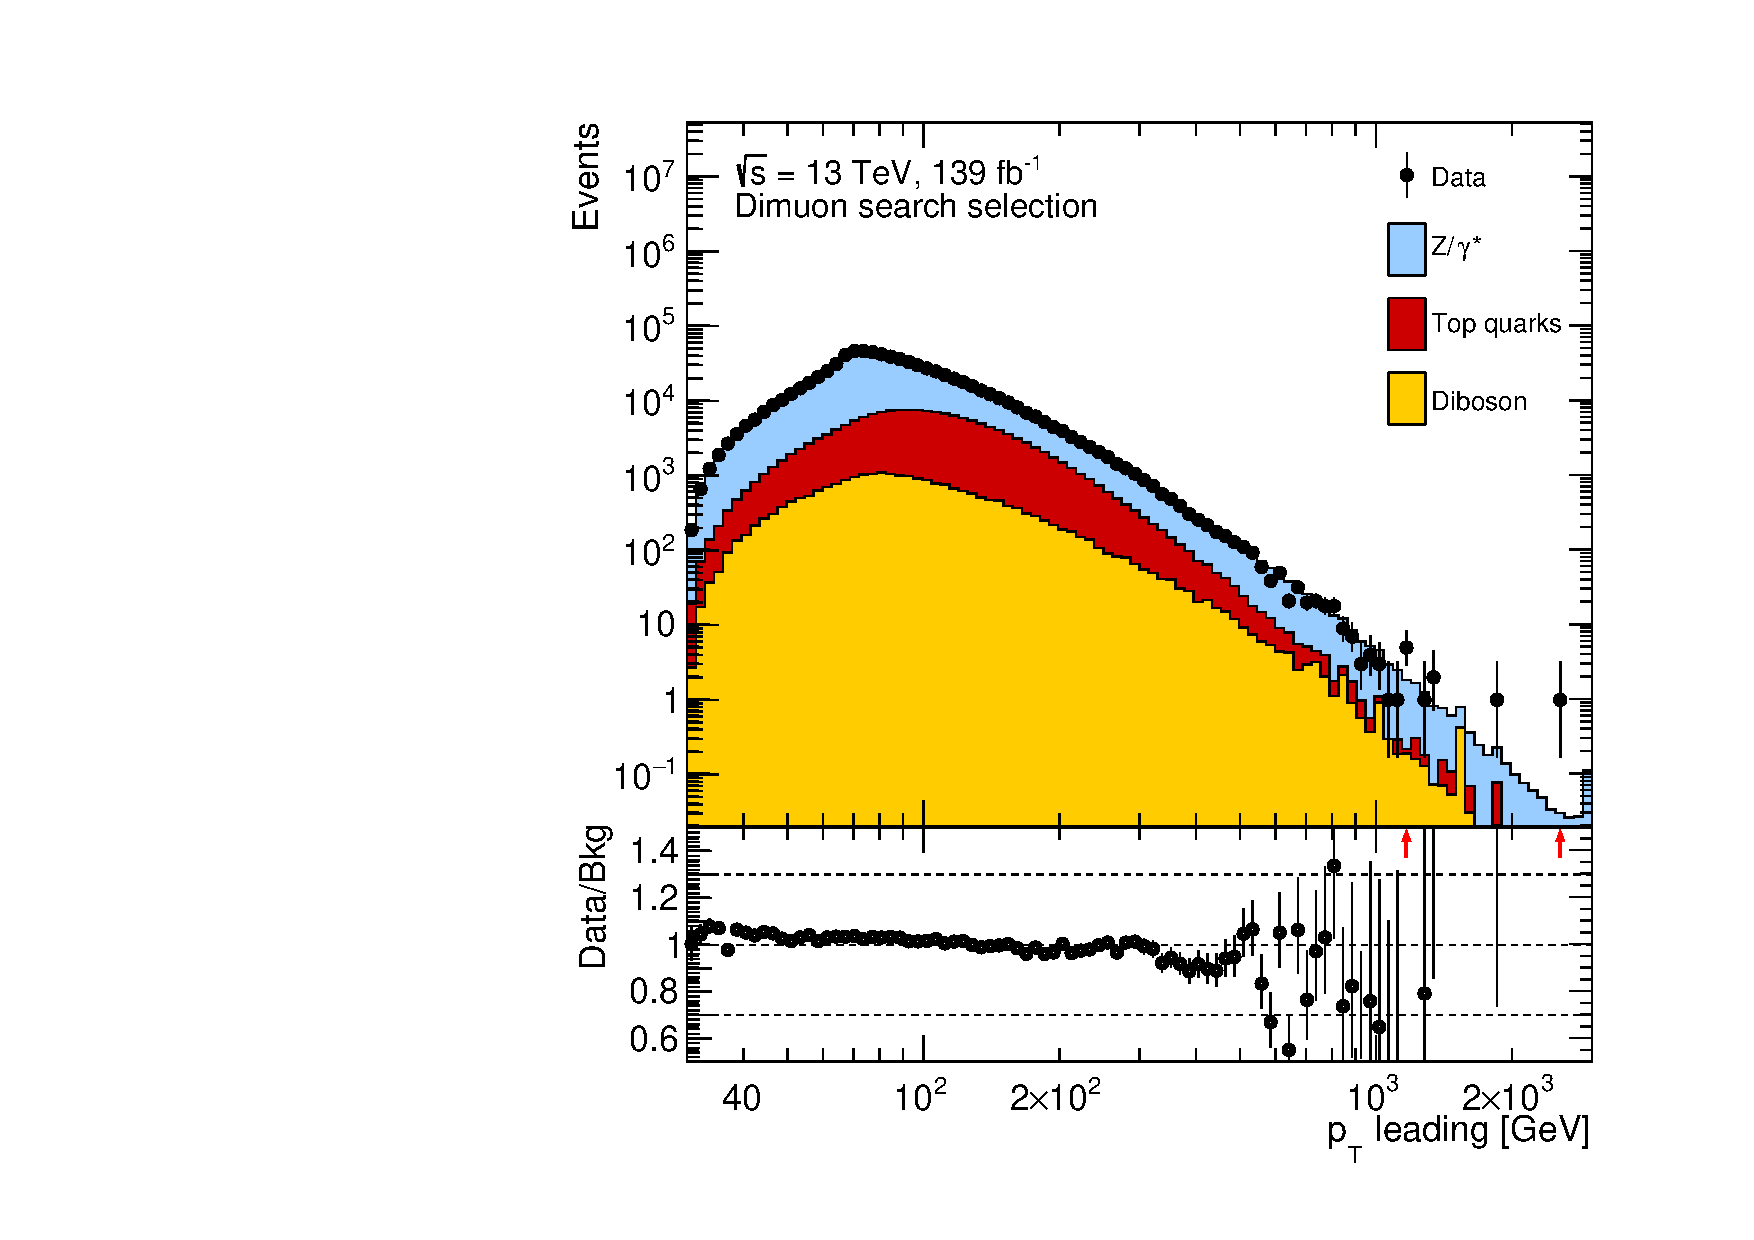
\includegraphics[width=\textwidth]{figures/analysis/datamc/dataMCcompare/uu_pt1_log100.pdf}
        \caption{}
        \label{fig:datamc:uupt1}
    \end{subfigure}
    \caption[$p_\mathrm{T}$ distribution of the leading lepton for the dilepton selections for the full $2015-18$ dataset and the respective MC campaigns.]{$p_\mathrm{T}$ distribution of the leading lepton for the dilepton selections for the full $2015-18$ dataset and the respective MC campaigns. The \ee channel is shown in (a) and \mumu channel in (b). Note that the fake electrons background component is not included in the \ee channel.}
    \label{fig:datamc:pt1}
\end{figure}

\begin{figure}[]
    \centering
    \begin{subfigure}[b]{0.49\textwidth}
        \centering
        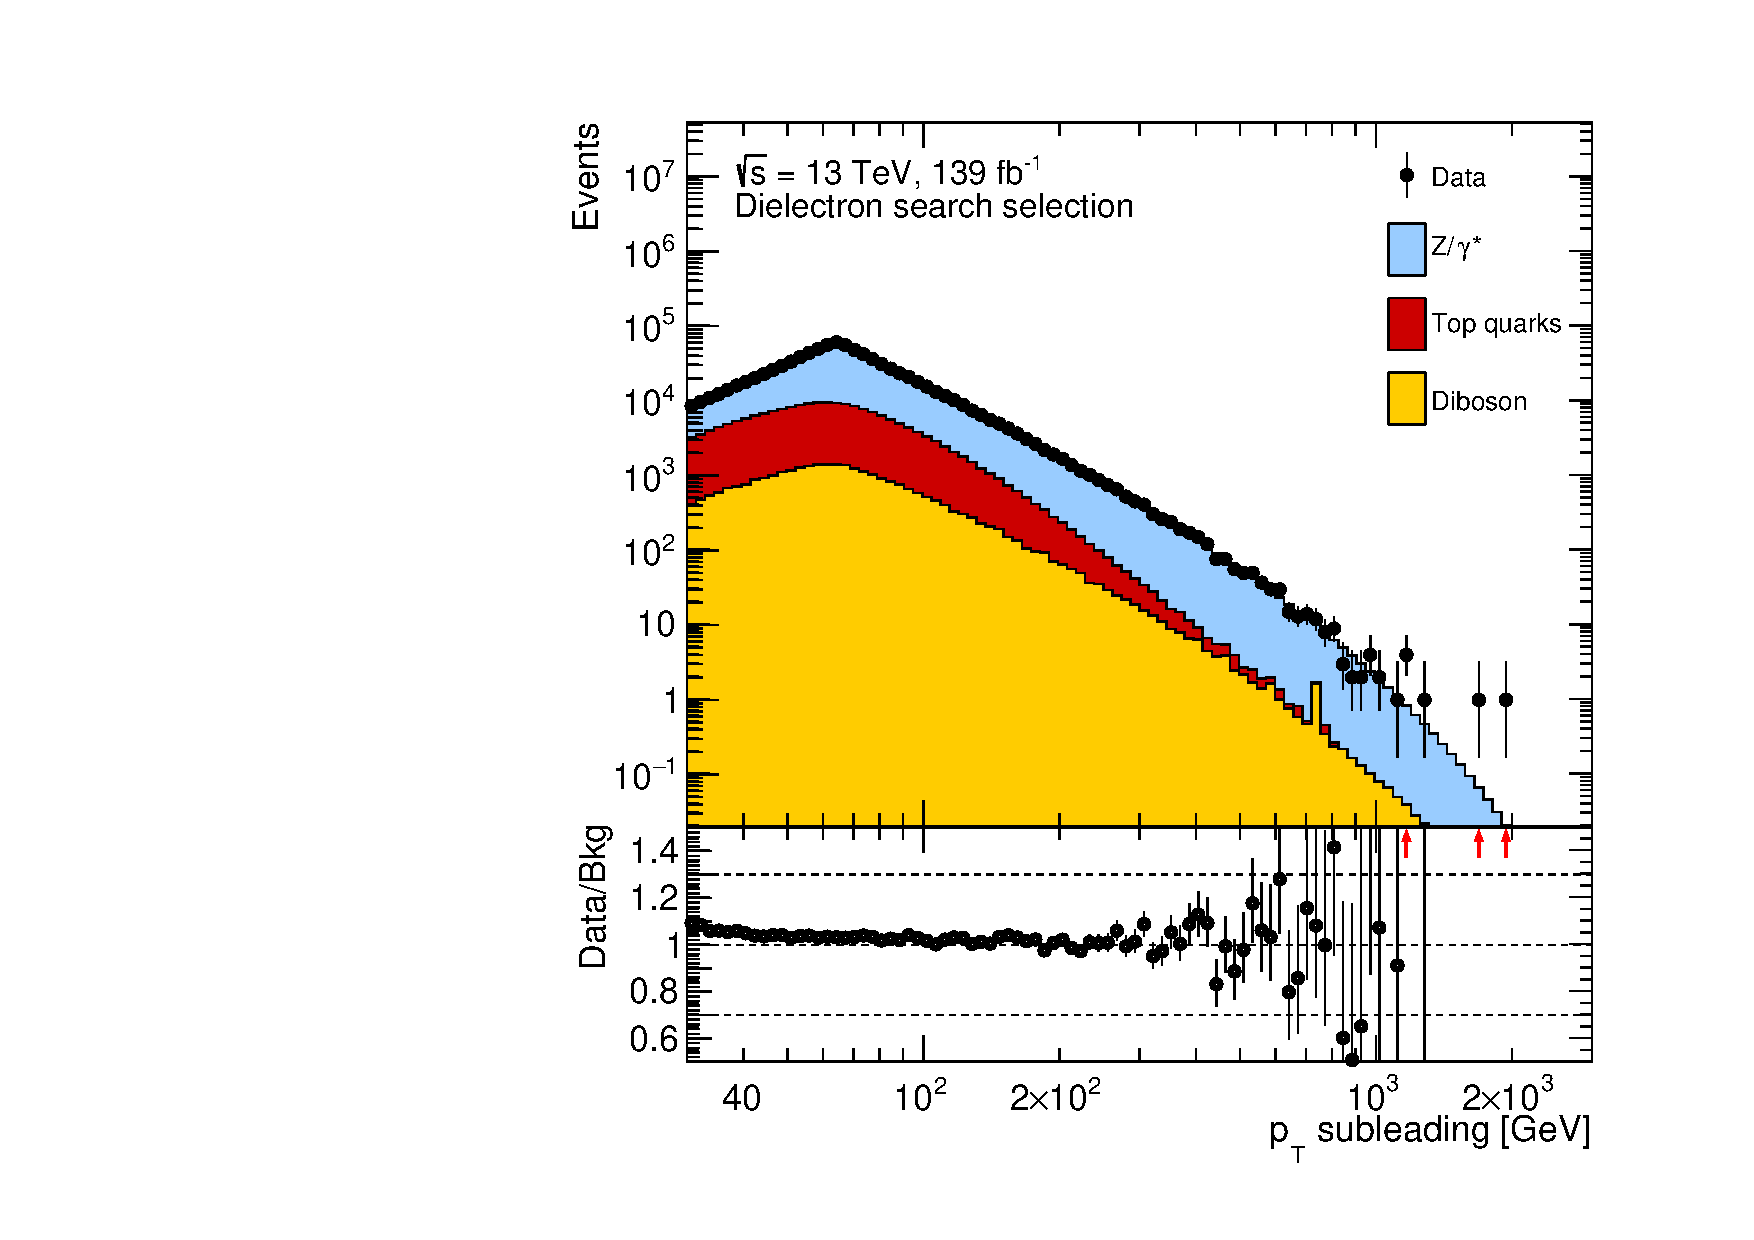
\includegraphics[width=\textwidth]{figures/analysis/datamc/dataMCcompare/ee_pt2_log100.pdf}
        \caption{}
        \label{fig:datamc:eept2}
    \end{subfigure}
    \begin{subfigure}[b]{0.49\textwidth}
        \centering
        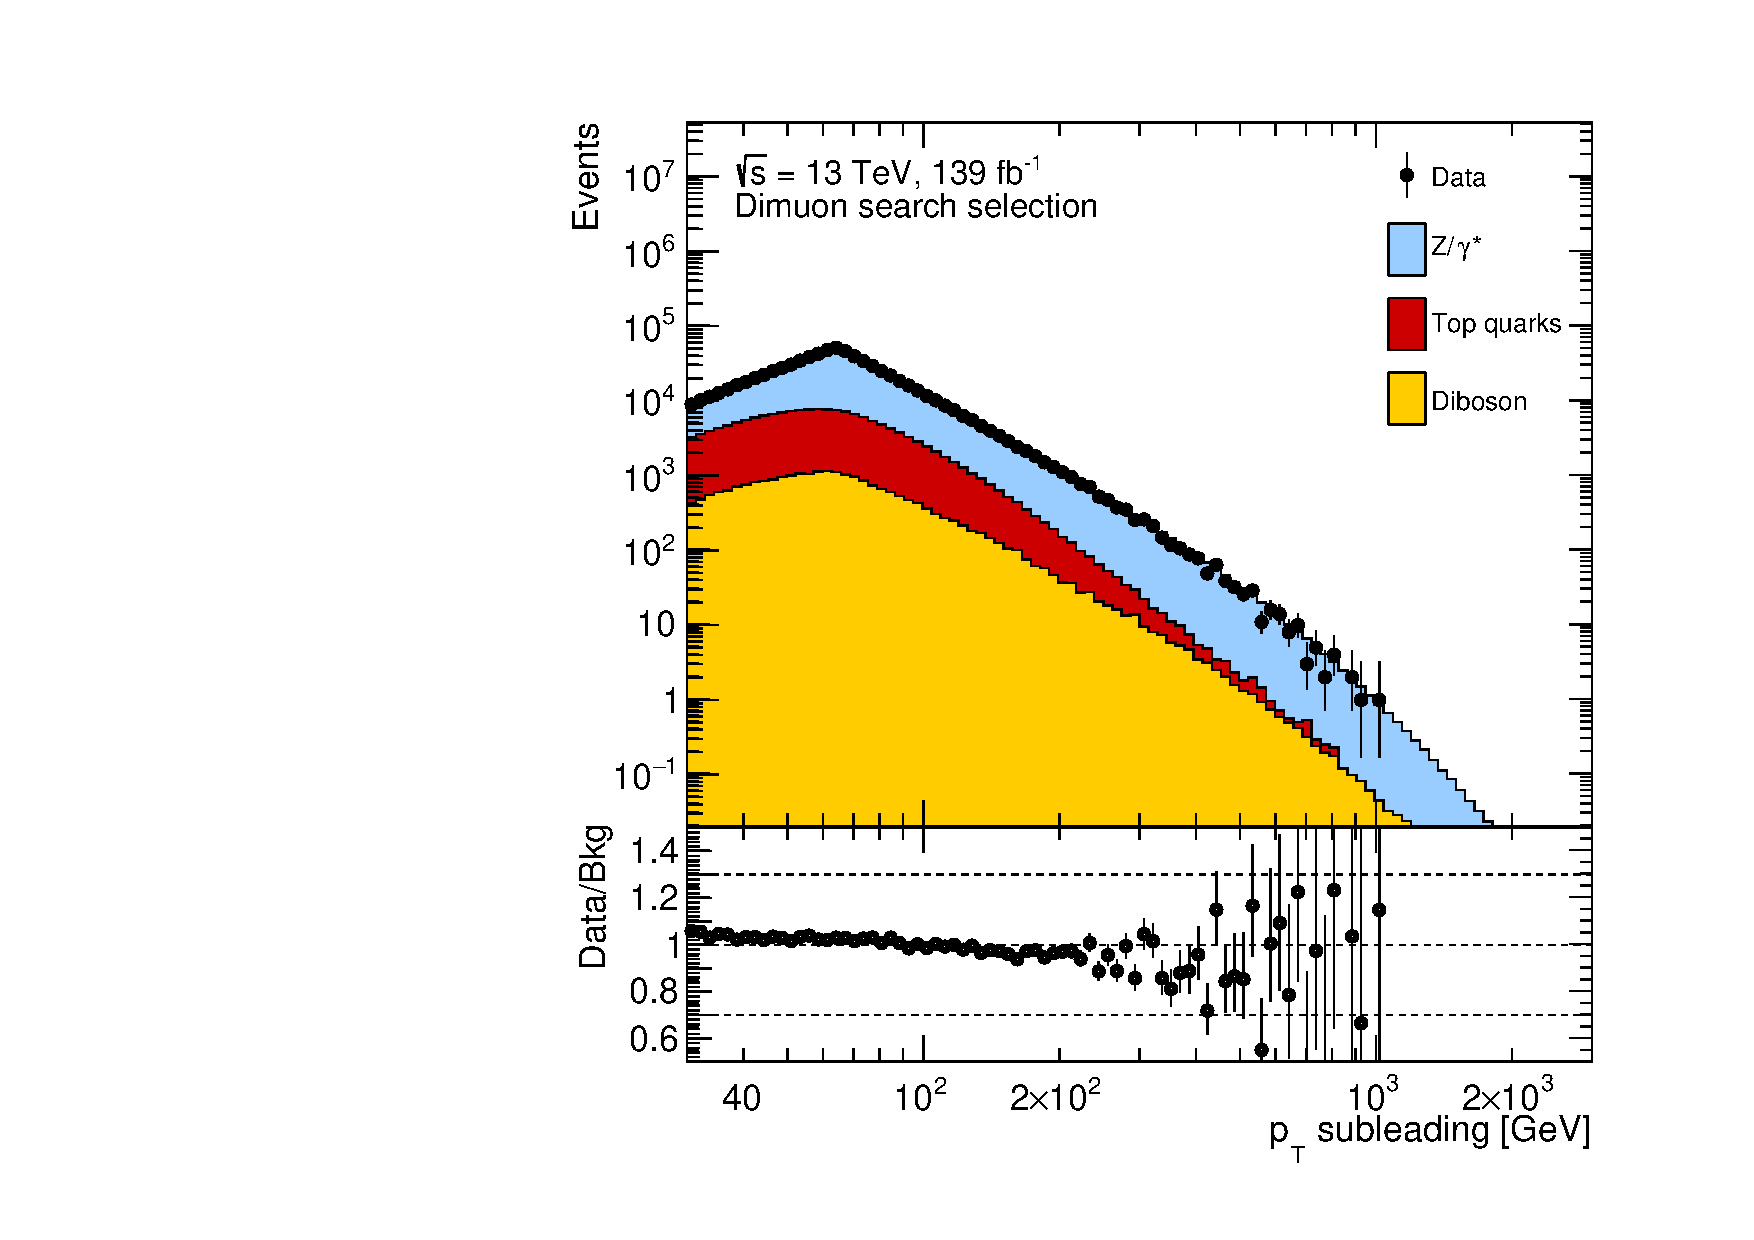
\includegraphics[width=\textwidth]{figures/analysis/datamc/dataMCcompare/uu_pt2_log100.pdf}
        \caption{}
        \label{fig:datamc:uupt2}
    \end{subfigure}
    \caption[$p_\mathrm{T}$ distribution of the subleading lepton for the dilepton selections for the full $2015-18$ dataset and the respective MC campaigns.]{$p_\mathrm{T}$ distribution of the subleading lepton for the dilepton selections for the full $2015-18$ dataset and the respective MC campaigns. The \ee channel is shown in (a) and \mumu channel in (b). Note that the fake electrons background component is not included in the \ee channel.}
    \label{fig:datamc:pt2}
\end{figure}

\begin{figure}[]
    \centering
    \begin{subfigure}[b]{0.49\textwidth}
        \centering
        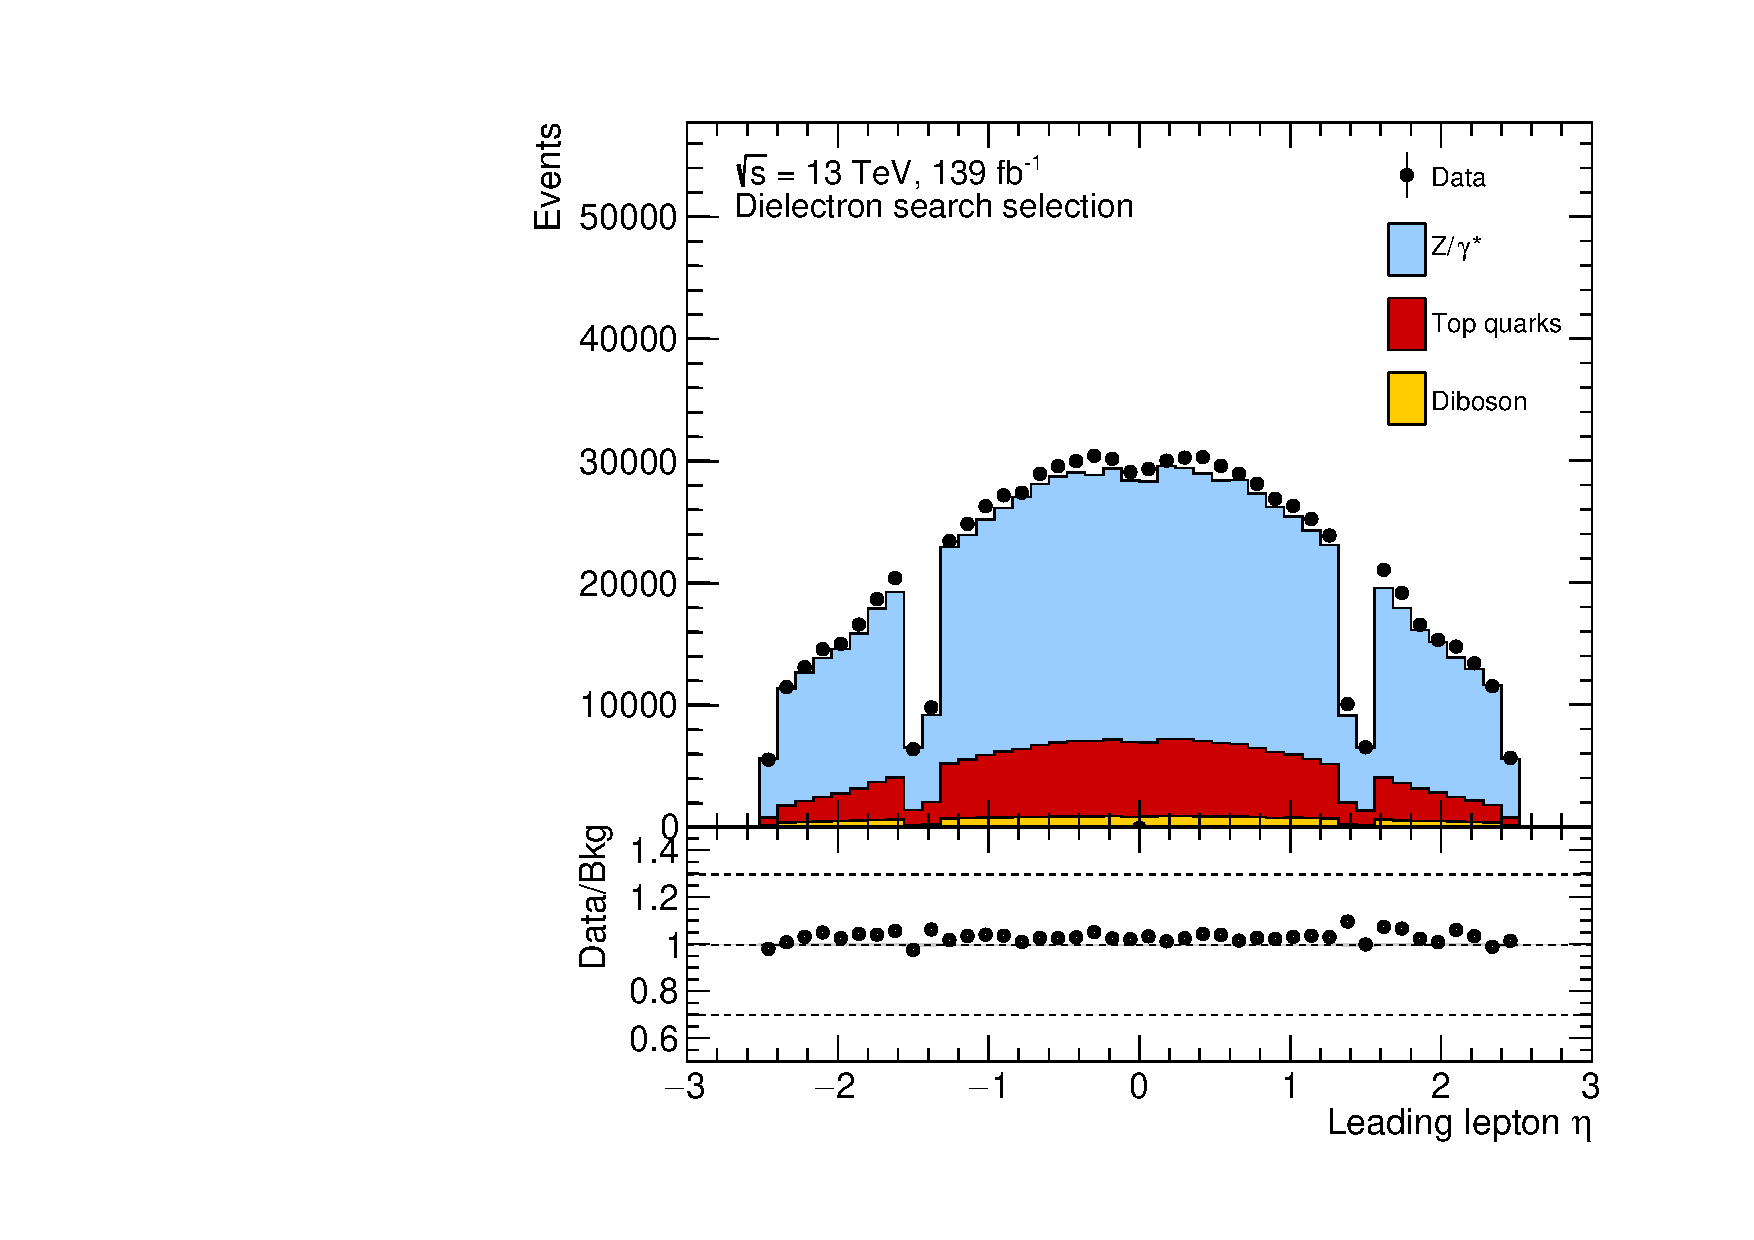
\includegraphics[width=\textwidth]{figures/analysis/datamc/dataMCcompare/ee_eta1.pdf}
        \caption{}
        \label{fig:datamc:eeeta1}
    \end{subfigure}
    \begin{subfigure}[b]{0.49\textwidth}
        \centering
        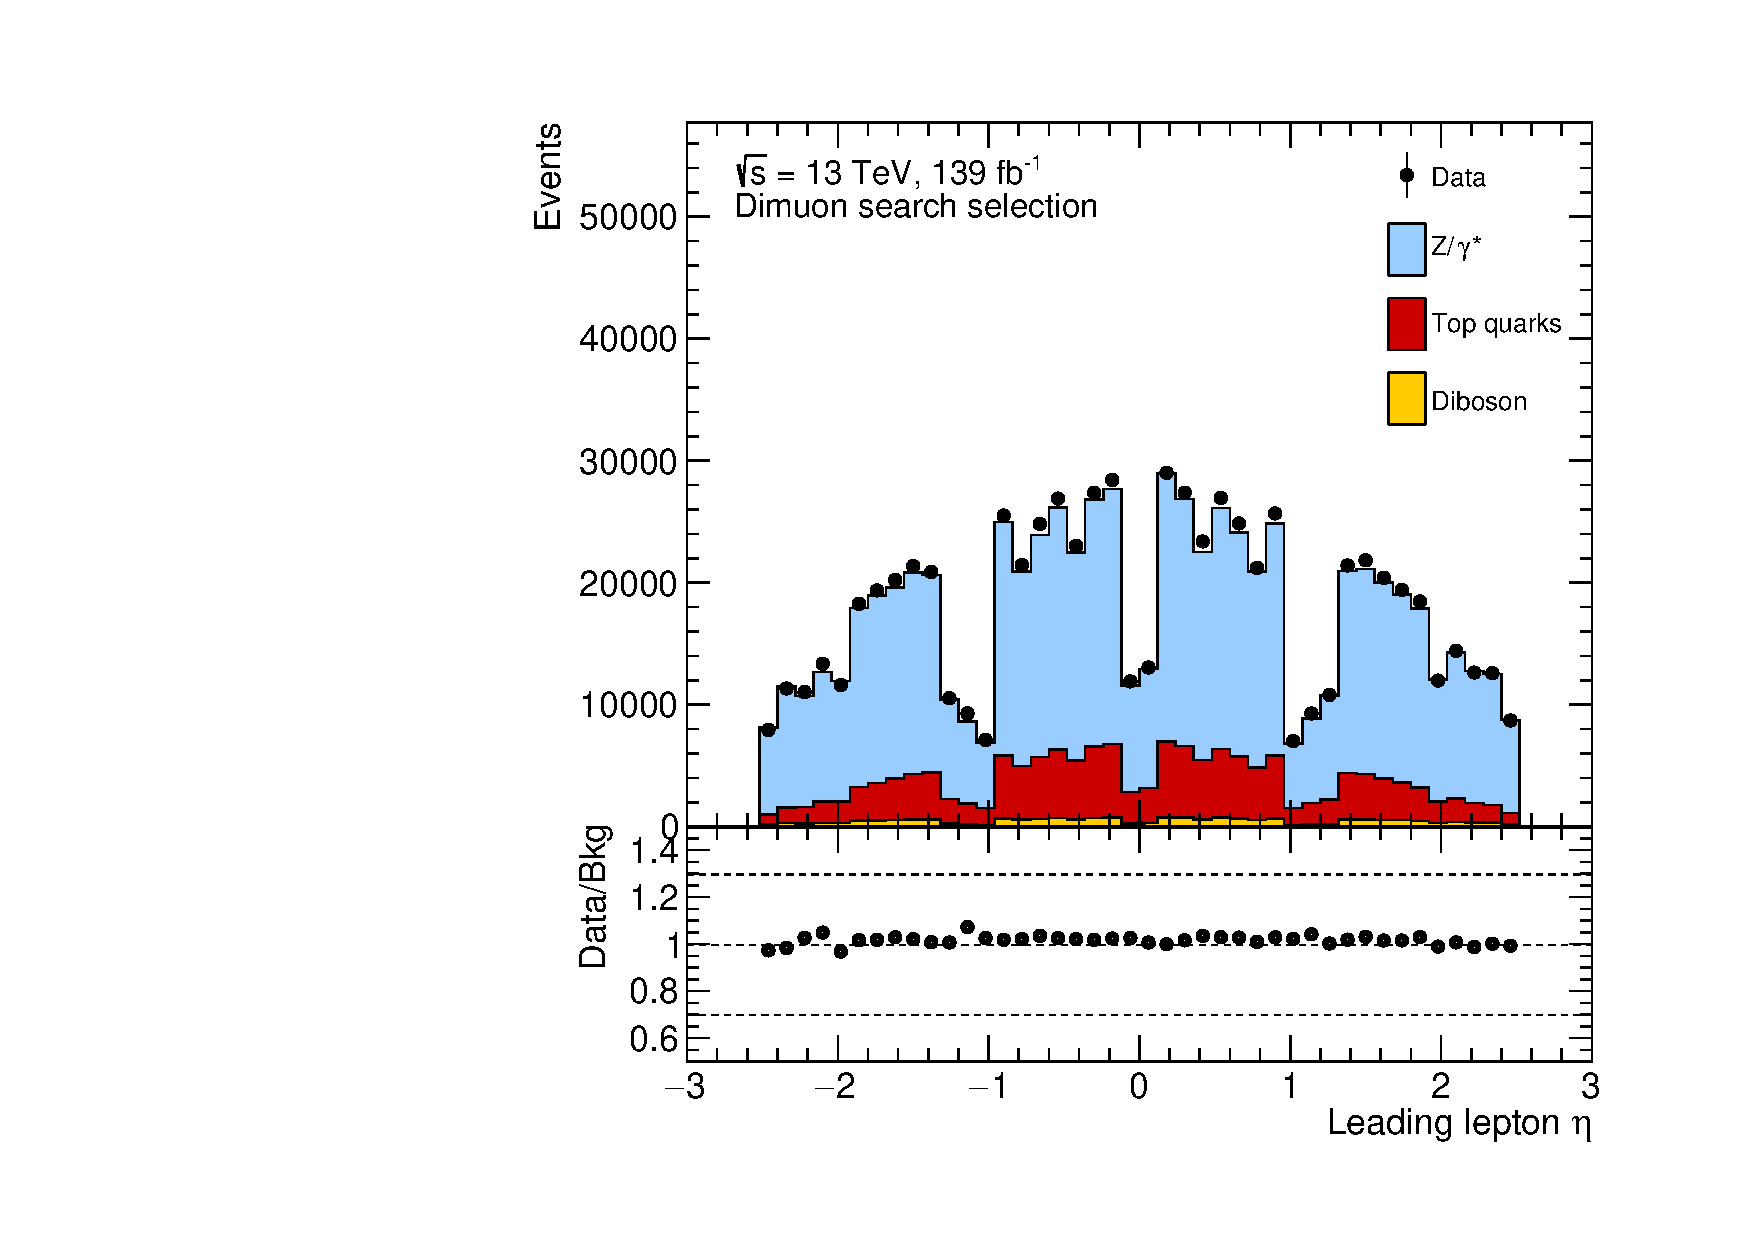
\includegraphics[width=\textwidth]{figures/analysis/datamc/dataMCcompare/uu_eta1.pdf}
        \caption{}
        \label{fig:datamc:uueta1}
    \end{subfigure}
    \caption[$\eta$ distribution of the leading lepton for the dilepton selections for the full $2015-18$ dataset and the respective MC campaigns.]{$\eta$ distribution of the leading lepton for the dilepton selections for the full $2015-18$ dataset and the respective MC campaigns. The \ee channel is shown in (a) and \mumu channel in (b). Note that the fake electrons background component is not included in the \ee channel.}
    \label{fig:datamc:eta1}
\end{figure}

\begin{figure}[]
    \centering
    \begin{subfigure}[b]{0.49\textwidth}
        \centering
        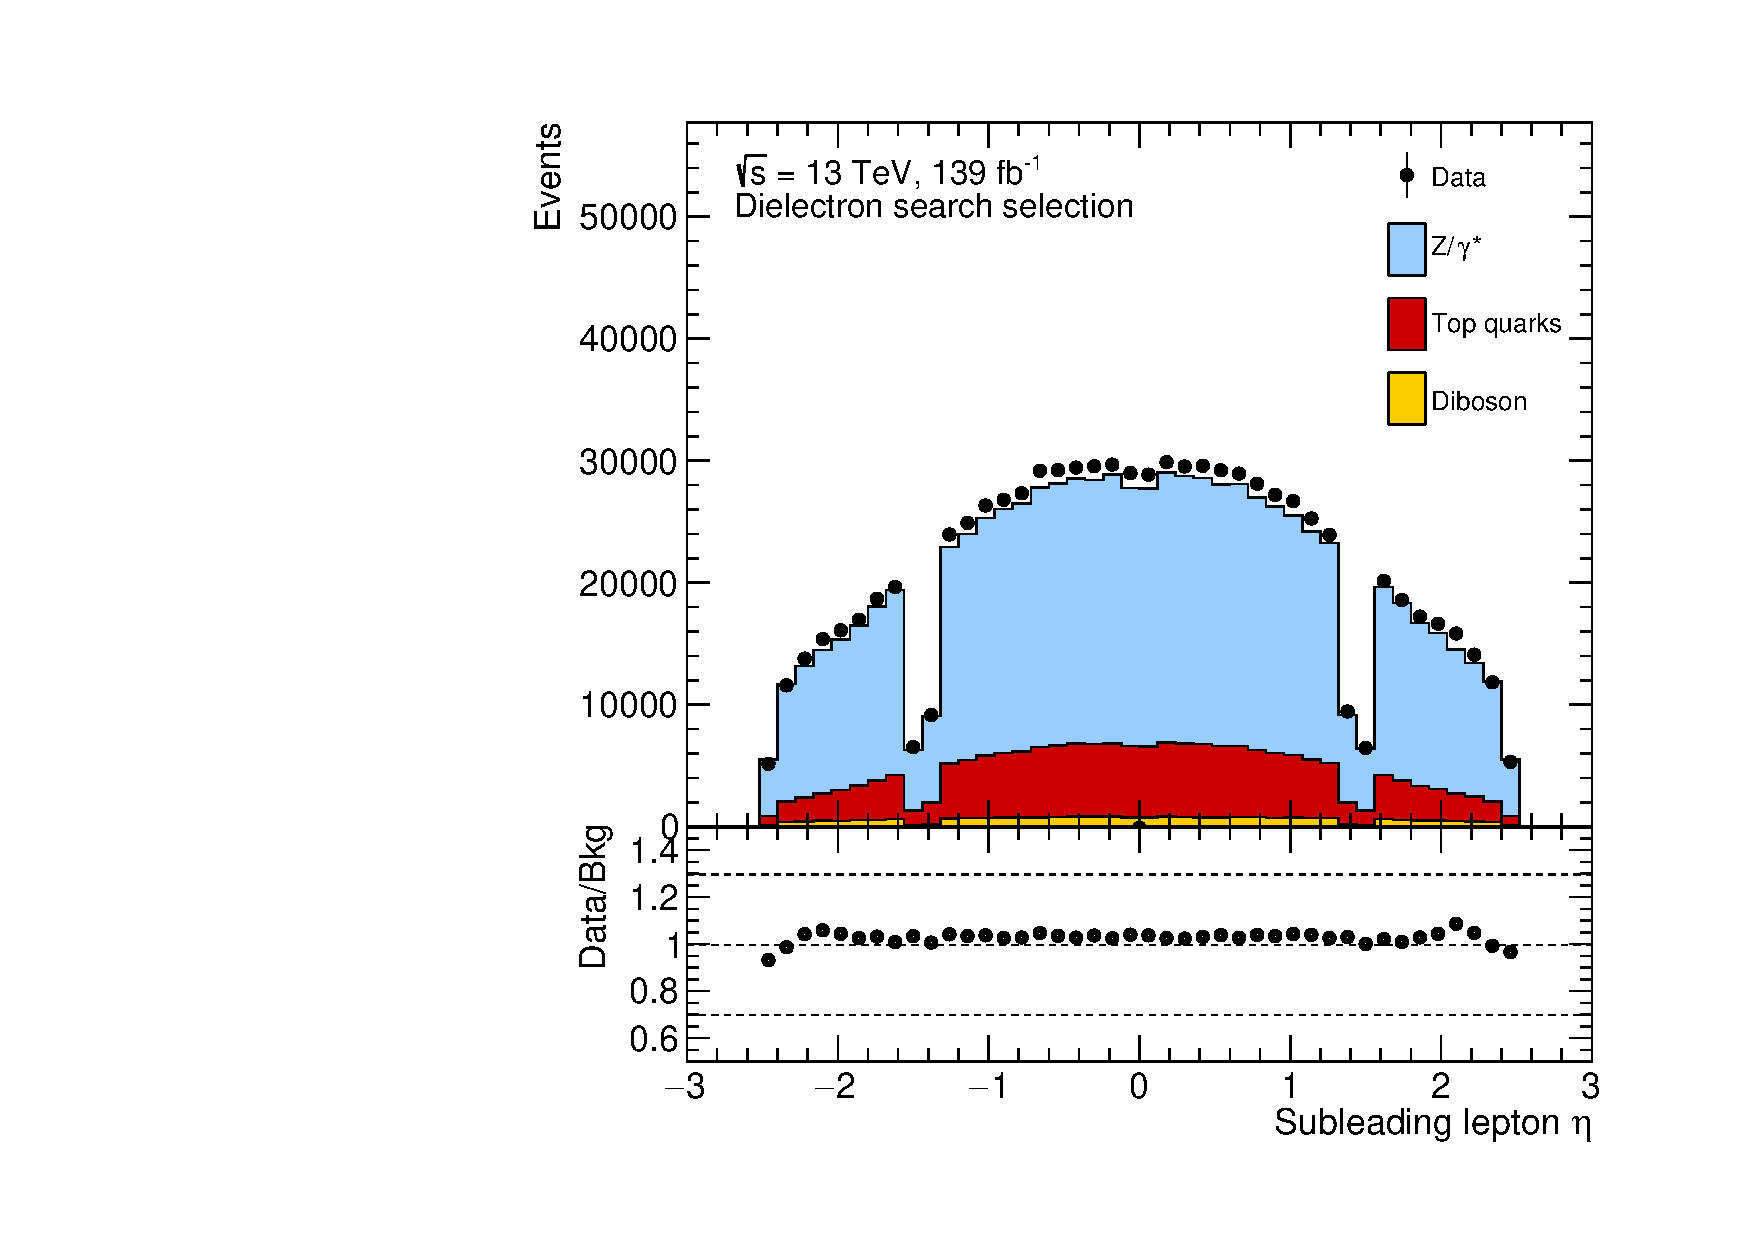
\includegraphics[width=\textwidth]{figures/analysis/datamc/dataMCcompare/ee_eta2.pdf}
        \caption{}
        \label{fig:datamc:eeeta2}
    \end{subfigure}
    \begin{subfigure}[b]{0.49\textwidth}
        \centering
        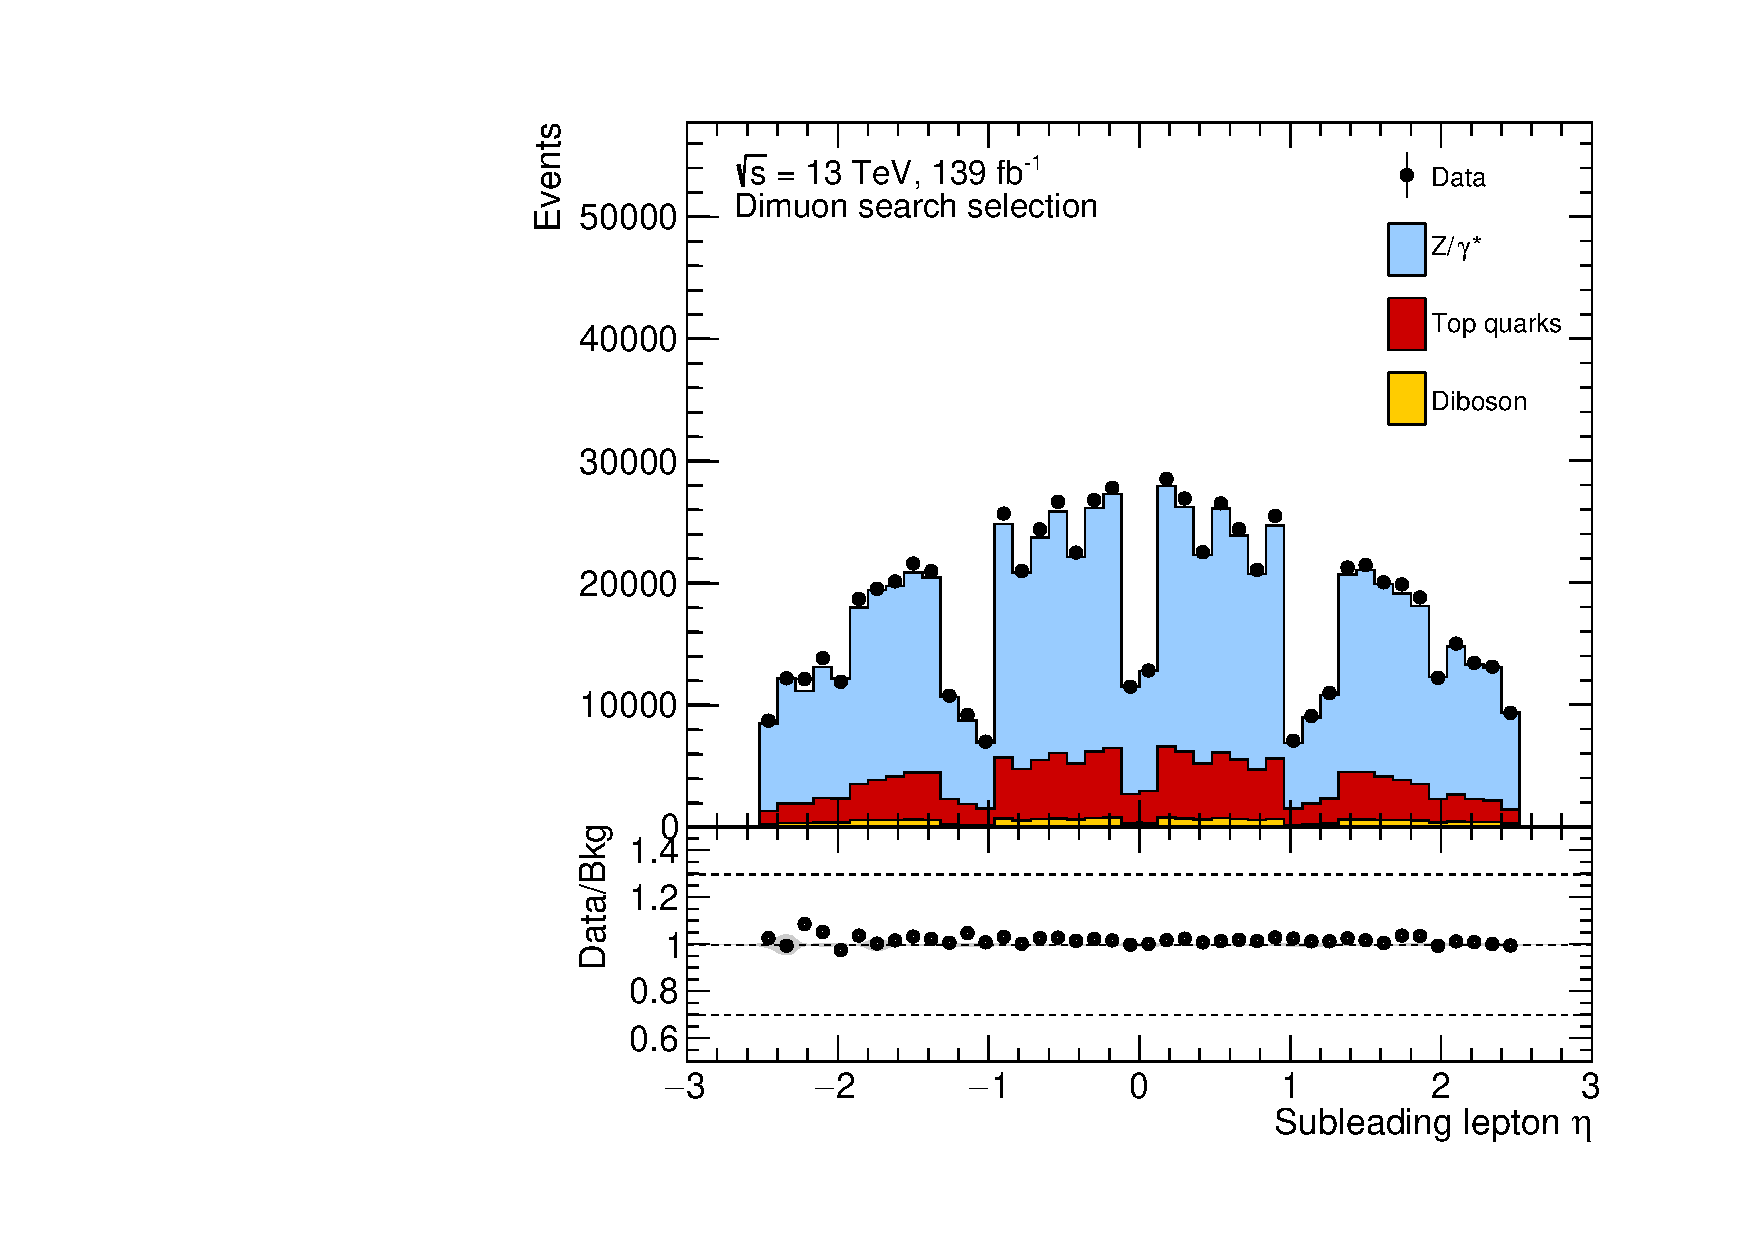
\includegraphics[width=\textwidth]{figures/analysis/datamc/dataMCcompare/uu_eta2.pdf}
        \caption{}
        \label{fig:datamc:uueta2}
    \end{subfigure}
    \caption[$\eta$ distribution of the subleading lepton for the dilepton selections for the full $2015-18$ dataset and the respective MC campaigns.]{$\eta$ distribution of the subleading lepton for the dilepton selections for the full $2015-18$ dataset and the respective MC campaigns. The \ee channel is shown in (a) and \mumu channel in (b). Note that the fake electrons background component is not included in the \ee channel.}
    \label{fig:datamc:eta2}
\end{figure}

\begin{figure}[]
    \centering
    \begin{subfigure}[b]{0.49\textwidth}
        \centering
        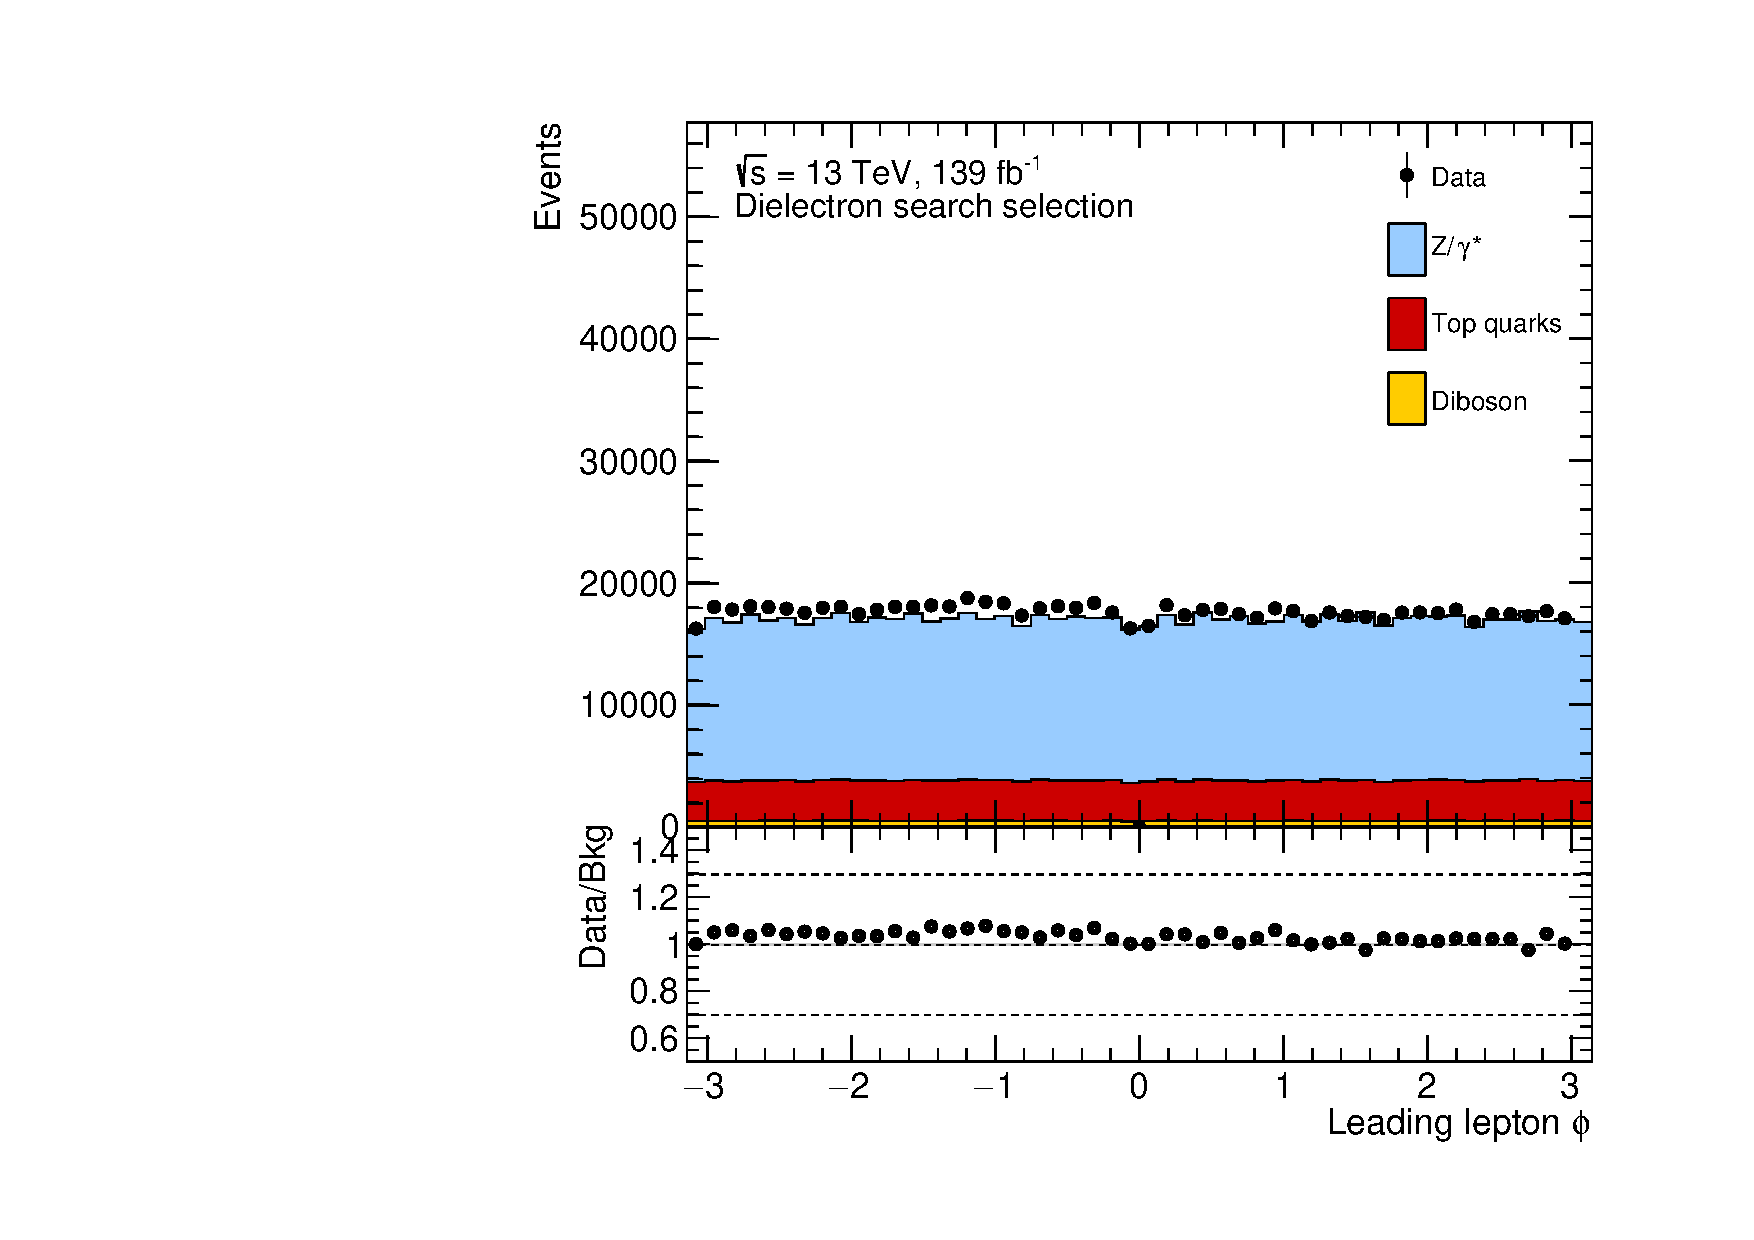
\includegraphics[width=\textwidth]{figures/analysis/datamc/dataMCcompare/ee_phi1.pdf}
        \caption{}
        \label{fig:datamc:eephi1}
    \end{subfigure}
    \begin{subfigure}[b]{0.49\textwidth}
        \centering
        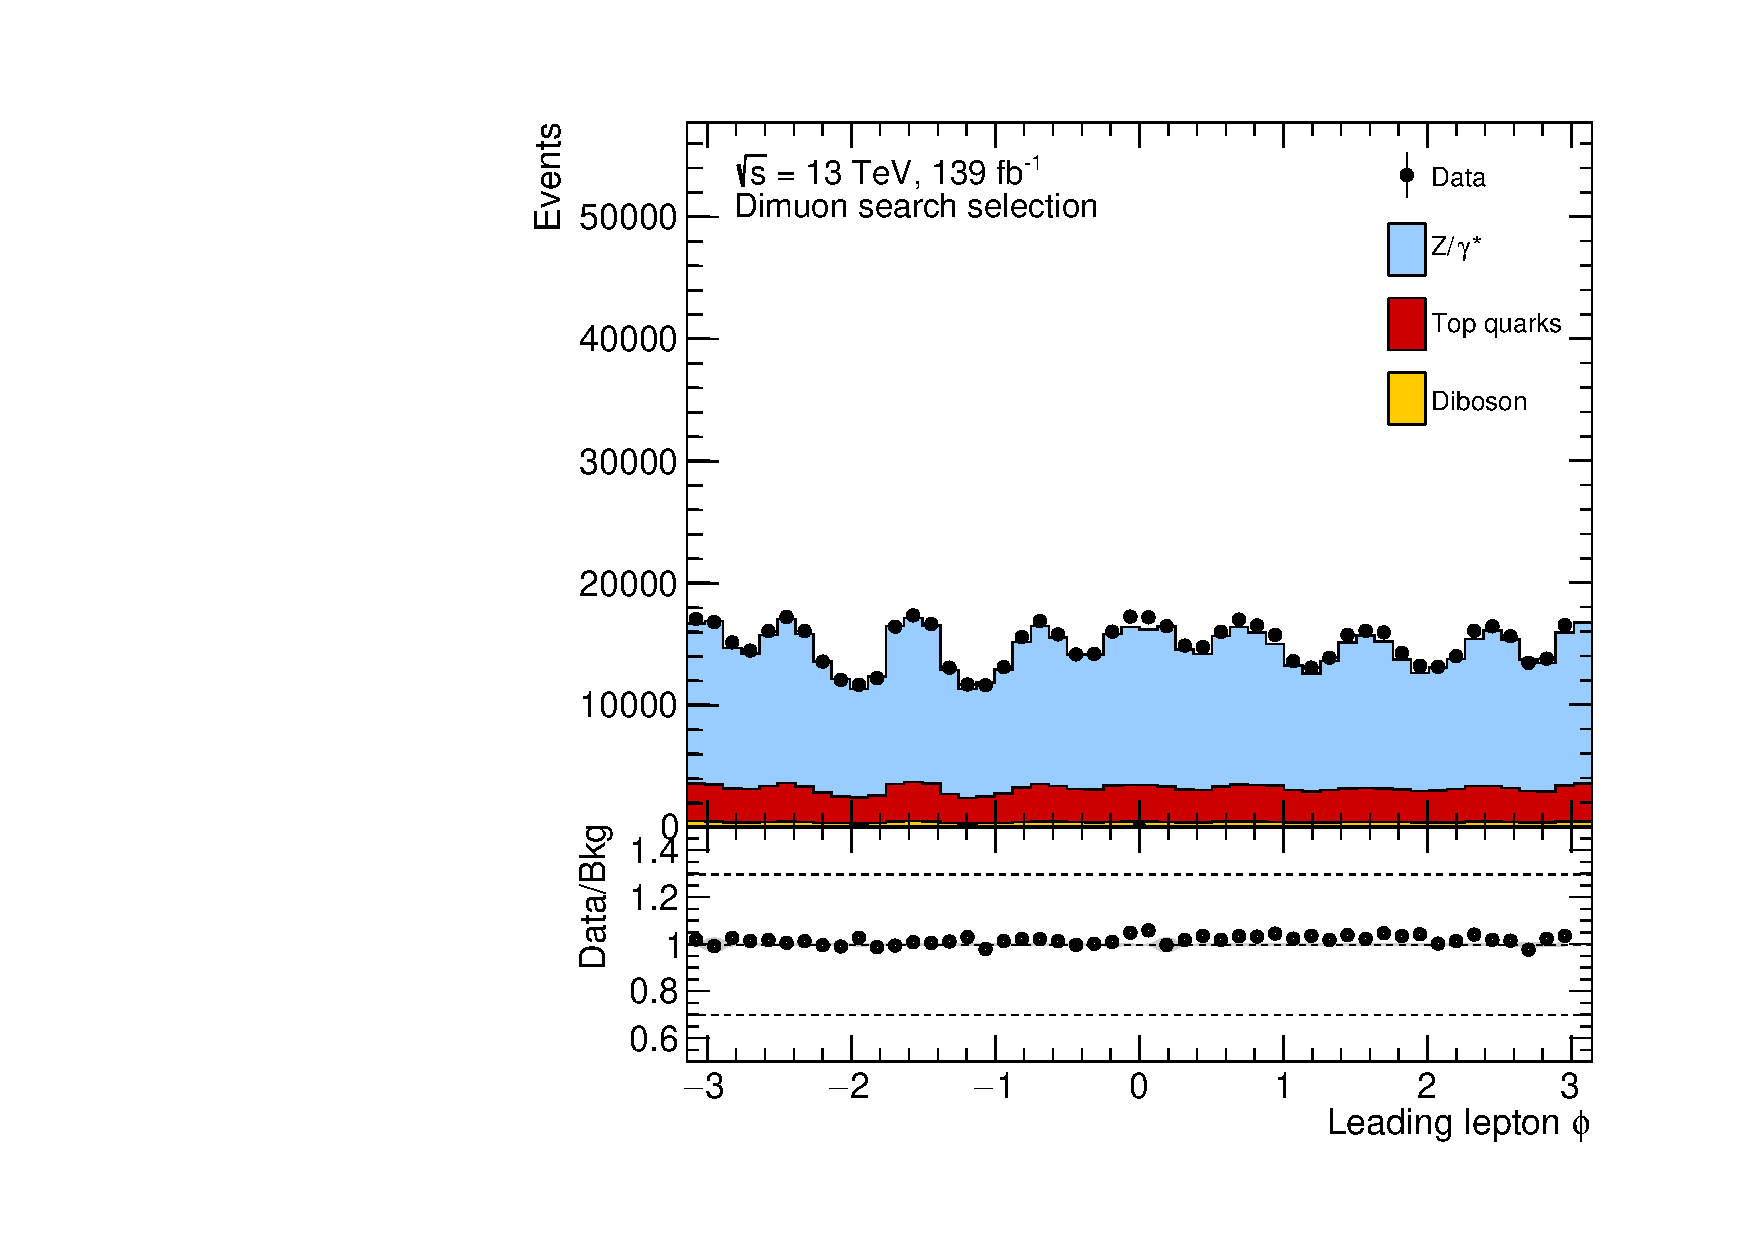
\includegraphics[width=\textwidth]{figures/analysis/datamc/dataMCcompare/uu_phi1.pdf}
        \caption{}
        \label{fig:datamc:uuphi1}
    \end{subfigure}
    \caption[$\phi$ distribution of the leading lepton for the dilepton selections for the full $2015-18$ dataset and the respective MC campaigns.]{$\phi$ distribution of the leading lepton for the dilepton selections for the full $2015-18$ dataset and the respective MC campaigns. The \ee channel is shown in (a) and \mumu channel in (b). Note that the fake electrons background component is not included in the \ee channel.}
    \label{fig:datamc:phi1}
\end{figure}

\begin{figure}[]
    \centering
    \begin{subfigure}[b]{0.49\textwidth}
        \centering
        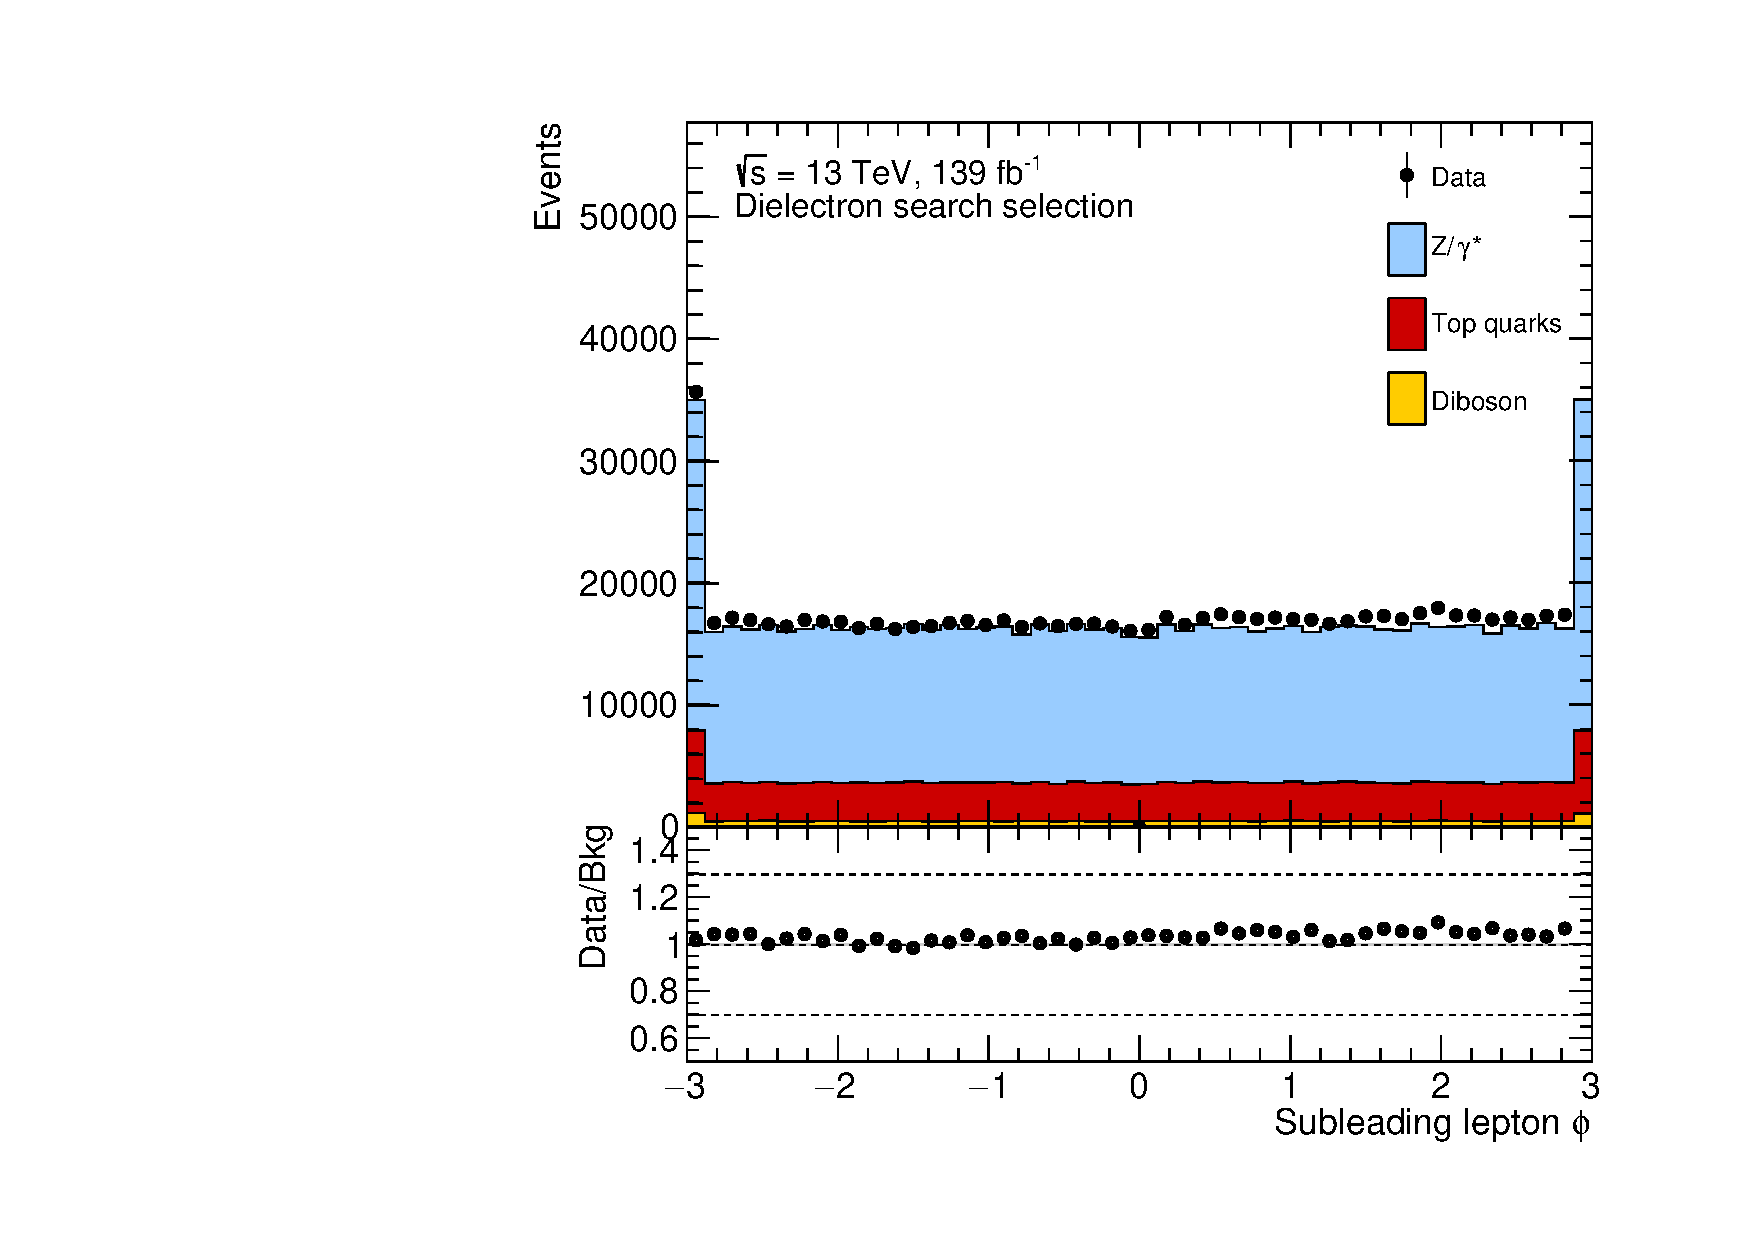
\includegraphics[width=\textwidth]{figures/analysis/datamc/dataMCcompare/ee_phi2.pdf}
        \caption{}
        \label{fig:datamc:eephi2}
    \end{subfigure}
    \begin{subfigure}[b]{0.49\textwidth}
        \centering
        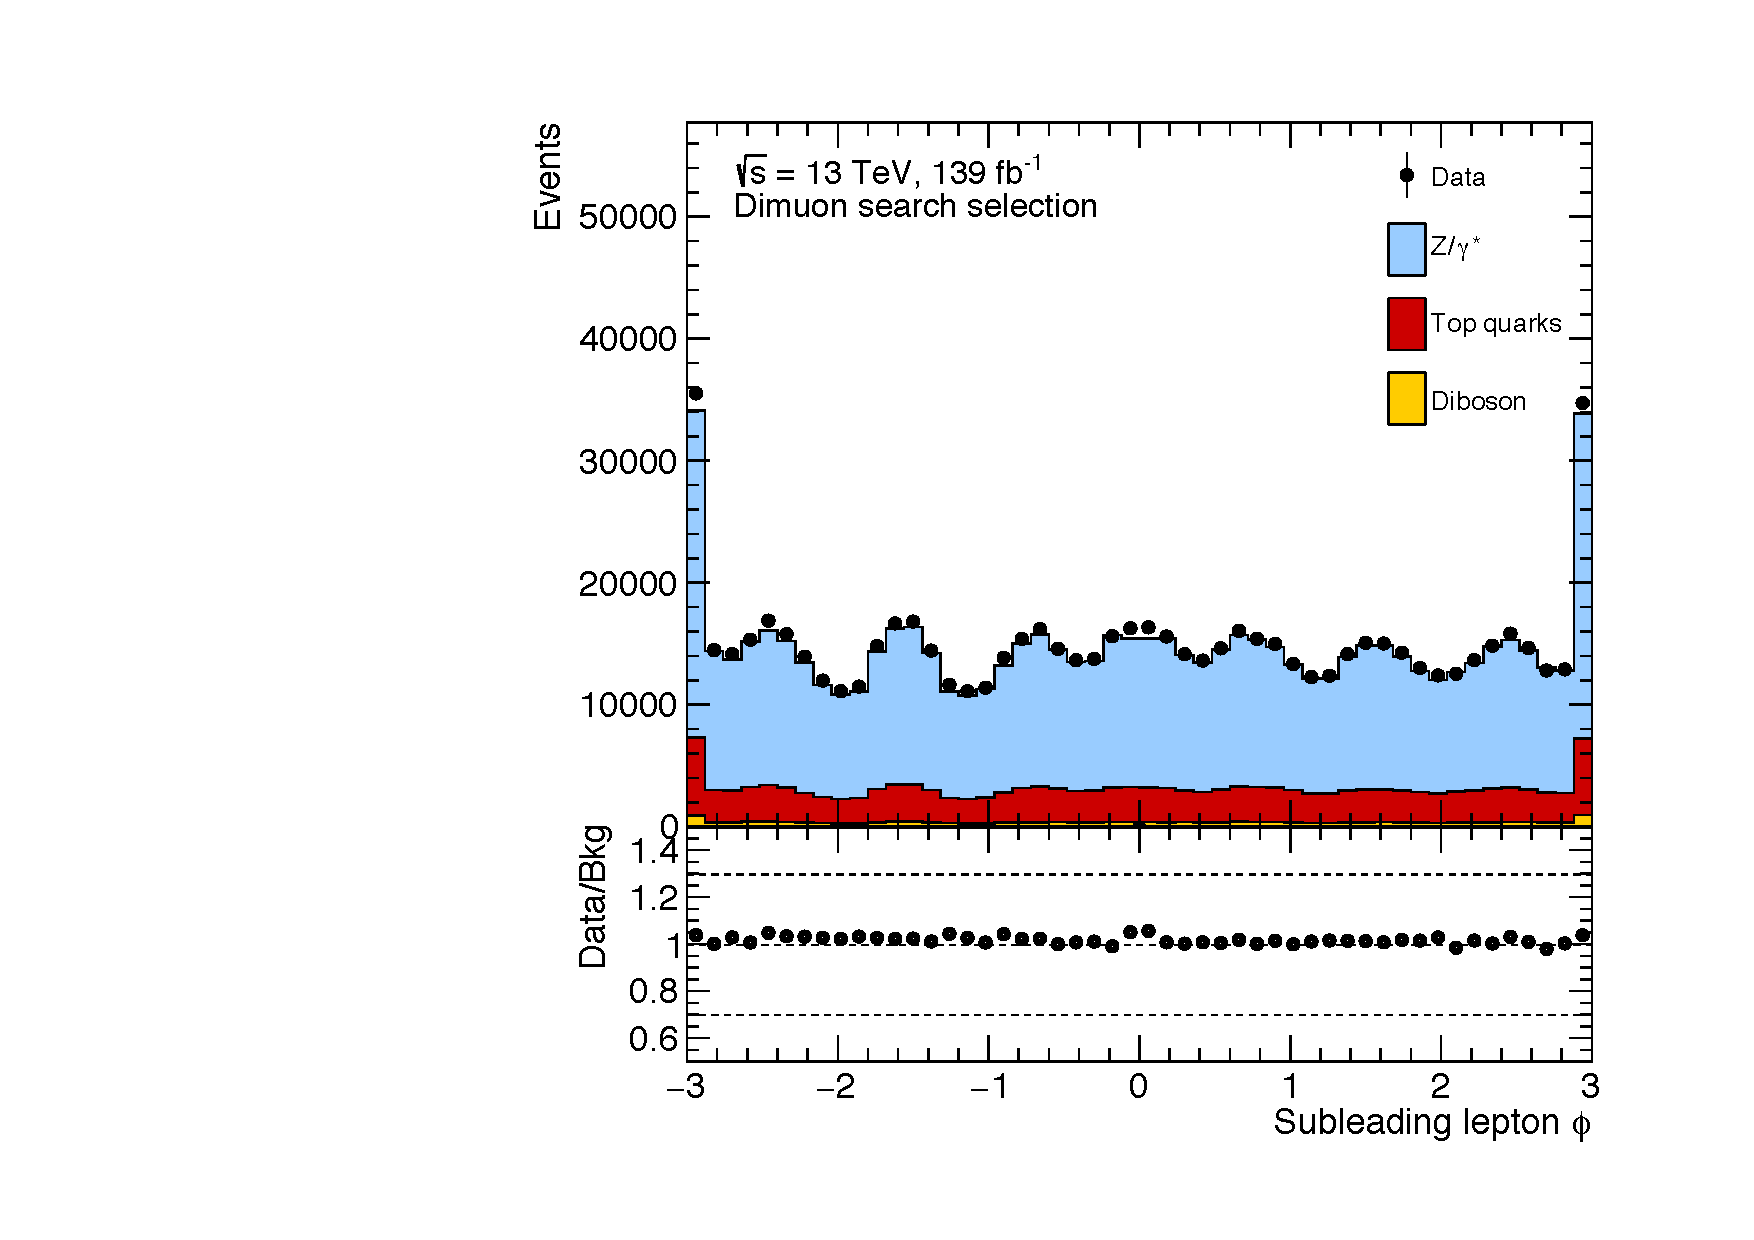
\includegraphics[width=\textwidth]{figures/analysis/datamc/dataMCcompare/uu_phi2.pdf}
        \caption{}
        \label{fig:datamc:uuphi2}
    \end{subfigure}
    \caption[$\phi$ distribution of the subleading lepton for the dilepton selections for the full $2015-18$ dataset and the respective MC campaigns.]{$\phi$ distribution of the subleading lepton for the dilepton selections for the full $2015-18$ dataset and the respective MC campaigns. The \ee channel is shown in (a) and \mumu channel in (b). Note that the fake electrons background component is not included in the \ee channel.}
    \label{fig:datamc:phi2}
\end{figure}
\clearpage

The comparison is mainly produced for illustrative purposes, since the MC background prediction is used only for the choice of functional fit. Nevertheless, a good agreement is between the data and MC expectation is required for the data-driven fit strategy. Furthermore, the comparisons allow for an early indication to issues that may have occurred when deciding on a selection. 

\section{Transfer functions}\label{sec:datamc:transfer}
The transfer function (TF) approach~\cite{Aad:2019fac}, based on an analytical parameterisation of the detector resolution, offers an alternative method to produce large statistics smooth DY and \ttbar samples. The method is used to overcome the limitations of insufficient MC statistics at invarant masses below \SI{2}{\tera\electronvolt}. The available MC samples for analysis of the $2015-16$ dataset~\cite{EXOT-2016-05} had statistical uncertainties that were compatible with the statistical uncertainty in data, resulting in a loss of sensitivity to new physics models. Complicated background smoothing techniques with functional fits were adopted in the analysis in an attempt to tackle the loss in sensitivity. 

The TF approach provides a smooth transformation between the truth and reconstruction level invariant mass spectrums. A functional form is not imposed on the TF, the transformation is analytically parametrised using the detector resolution. The electron and muon channel require separate TFs due to the different reconstruction properties of the two channels. 

\subsection{Overview}
The transition between a known truth spectrum, $S_t(m_{\ell\ell}^{truth})$, and an unknown reconstructed spectrum, $S_r(m_{\ell\ell}^{reco})$, is be parametrised by a TF, $P(m_{\ell\ell}^{reco} \mid m_{\ell\ell}^{truth})$. $P(m_{\ell\ell}^{reco} | m_{\ell\ell}^{truth})$ describes the probability to reconstruct an event at invariant mass of $m_{\ell\ell}^{reco}$ for events with truth mass $m_{\ell\ell}^{truth}$ that passes the selection. Full simulation MC is used to construct the TFs, where additional smoothing of the MC can be done via a fit with the $P(m_{\ell\ell}^{reco} \mid m_{\ell\ell}^{truth})$. The truth invariant mass spectrum is obtained from a very large truth-only MC samples. Larger samples are able to be produced at truth-level compared to fully reconstructed samples due to significantly smaller CPU times and disk space required to produce them. The truth-only sample is produced such that it is produced at luminosity 55 times larger than the available dataset. The reconstruction level spectrum is then obtained by the following convolution: 
\begin{equation}\label{eq:TF_generalConv}
	S_r(m_{\ell\ell}^{reco}) = P(m_{\ell\ell}^{reco} \mid m_{\ell\ell}^{truth}) \otimes \left[ S_t(m_{\ell\ell}^{truth}) \cdot A\varepsilon(m_{\ell\ell}^{truth})) \right], 
\end{equation}
where $A\varepsilon(m_{\ell\ell}^{truth}))$ is the acceptance times efficiency. $A\varepsilon(m_{\ell\ell}^{truth}))$ is the probability that a event with truth invariant mass passes the selection. It is calculated by taking the fraction of events accepted in a truth invariant mass bin and the total number of generated events in that bin. 

\subsection{Parametrisation of detector response}
The TFs are obtained by fitting the detector response, $P(\mathcal{R} \mid m_{\ell\ell}^{truth})$, with a simultaneous fit on 200 $m_{\ell\ell}^{truth}$ bins. The detector response, $\mathcal{R}$, is used as the main variable in the fit due to it's mean value expected to be zero for each truth bin, and is defined as $\mathcal{R} = (m_{\ell\ell}^{reco} - m_{\ell\ell}^{truth}/ m_{\ell\ell}^{truth})$. To capture the response in the tail regions, a range of $R \in [-0.2,0.1]$ and $R \in [-0.75,0.75]$ is fitted for the electron and muon channels respectively. The range is chosen to cover the effects of the detector resolutions in the low and high invariant mass regions for both channels. 

A sum of a Gaussian and Crystal-ball function is used to model $P(\mathcal{R} \mid m_{\ell\ell}^{truth})$ after several functions were tested. The Gaussian, G, component of the function is chosen to model the main peak of the detector response, whereas the longer tails of the Crystal-Ball, CB, models the tails of the detector response. The tails of the response in the electron channel are caused by electromagnetic radiation due to Bremsstrahlung. In the muon channel the tails are a result of poorly reconstructed muons. The function is defined as: 
\begin{equation}\label{eq:TF_responseParam}
    P(\mathcal{R}) = \kappa \cdot \mathrm{CB}(\mathcal{R}| \mu_\mathrm{CB}, \sigma_\mathrm{CB}, \alpha_\mathrm{CB}, n_\mathrm{CB}) + (1 - \kappa) \cdot \mathrm{Gauss}(\mathcal{R}| \mu_\mathrm{G}, \sigma_\mathrm{G}).
\end{equation}
where,  $\mu_\mathrm{CB}$ and $\mu_\mathrm{G}$ are the mean values of the CB and G, respectively. $\mu_i$ is expected to be zero due the definition of $\mathcal{R}$. $\sigma_\mathrm{CB}$ and $\sigma_\mathrm{G}$ are the width parameters of the CB and Gaussian components, respectively. $\alpha_\mathrm{CB}$ is the cut-off for the CB after which the Gaussian behaviour is replaced by a power-law. $n_\mathrm{CB}$ is the exponent of the power-law and $\kappa$ is the fraction of the CB function in the total probability density function.

The parameters of the response functions are then parameterised as a function of $m_{\ell\ell}^{truth}$ to allow for simultaneous fits in all $m_{\ell\ell}^{truth}$ regions. Initial values for the parameters are obtained by fitting the detector response in single $m_{\ell\ell}^{truth}$ regions. The simultaneous fits are then performed and the final detector response is obtained as:
\begin{equation}\label{eq:TF_responseTransformation}
    \begin{aligned}
        & \mu_i(m_{\ell\ell}^{truth}) \to \mu_i'(m_{\ell\ell}^{truth}) = \left(\mu_i(m_{\ell\ell}^{truth}) \cdot m_{\ell\ell}^{truth}\right) + m_{\ell\ell}^{truth}, \\
        & \sigma_i(m_{\ell\ell}^{truth}) \to \sigma_i'(m_{\ell\ell}^{truth}) = \sigma_i(m_{\ell\ell}^{truth}) \cdot m_{\ell\ell}^{truth},
    \end{aligned}
\end{equation}

\clearpage